%% -*- coding: utf-8; -*-

\documentclass[
%  draft,
master,
brazilian
]{ThesisPUC_back}

\renewcommand{\floatpagefraction}{.9}
\renewcommand{\topfraction}{.9}
\renewcommand{\bottomfraction}{.9}
\renewcommand{\textfraction}{.01}

%%% Personal Commands
\renewcommand{\quote}[1]{``#1''}
%%%

\usepackage{microtype}

%\hyphenation{ma-lhas}
%\hyphenation{vi-su-a-li-za-ção}
%%%
%%% Additional Packages
%%%

  %% \usepackage[brazilian]{babel}      %% in ThesisPUC.cls
  %% \usepackage[utf8]{inputenc}        %% .
  %% \usepackage[T1]{fontenc}           %% .
  %% \usepackage{lmodern}               %% .
  %% \usepackage[pdftex]{graphicx}	%% .
\usepackage{gensymb}
  \usepackage{tabularx}
  \usepackage{multirow}
  \usepackage{multicol}
  \usepackage{colortbl}
  \usepackage[%
    dvipsnames,
    svgnames,
    x11names,
    fixpdftex
  ]{xcolor}
  \usepackage{numprint}
  \usepackage{textcomp}
  \usepackage{booktabs}
  \usepackage{amsmath}
  \usepackage{enumitem}
  \usepackage{amssymb}
  \usepackage{textcomp}
  \usepackage{float}
% \usepackage{etoolbox}

%% numprint 
\npthousandsep{.}
\npdecimalsign{,}

%% ThesisPUC option
%% \tablesmode{figtab} %% [nada, fig, tab ou figtab]


%%%
%%% Counters
%%%

%% uncomment and change for other depth values
%\setcounter{tocdepth}{1}
\setcounter{lofdepth}{1}
%% \setcounter{lotdepth}{3}
%% \setcounter{secnumdepth}{3}


%%%
%%% New commands and other global definitions
%%%

%\input{defs}


%%%
%%% Misc.
%%%

\usecolour{true}


%%%
%%% Titulos
%%%

\author{Rustam Câmara Mesquita}
\authorR{Mesquita, Rustam}

\advisor{Waldemar Celes Filho}{Prof.}
\advisorR{Celes Filho, Waldemar}

\title{Geração Semiautomática de Função de Transferência para Realce de Fronteiras Baseada em Derivadas Médias}

\titleuk{Semi-Automatic Generation of Transfer Function for Boundary Highlight Based on Average Derivatives}

%% \subtitulo{Aqui vai o subtitulo caso precise}

\day{16}
\month{Março}
\year{2018}

\city{Rio de Janeiro}
\CDD{004}
\department{Informática}
\program{Informática}
\school{Centro Técnico Científico}
\university{Pontifícia Universidade Católica do Rio de Janeiro}
\uni{PUC-Rio}


%%%
%%% Jury
%%%

\jury{%
	\jurymemberext{Luiz Henrique de Figueiredo}{Prof.}
	{IMPA}{}
	\jurymember{Marcelo Gattass}{Prof.}
	{Departamento de Informática}{PUC-Rio}
	\jurymember{Helio Côrtes Vieira Lopes}{Prof.}
	{Departamento de Informática}{PUC-Rio}
	\schoolhead{José Eugenio Leal}{Prof.}
}


%%%
%%% Resume
%%%

\resume{%
  Graduado em Engenharia da Computação pela Pontifícia Universidade Católica do Rio de Janeiro (Rio de Janeiro, Brasil) em 2014, tornou-se bolsista de mestrado associado ao Instituto Tecgraf de Desenvolvimento de Software Técnico-Científico da PUC-Rio em 2015, onde iniciou seu desenvolvimento profissional em computação gráfica. Durante o mestrado, direcionou sua pesquisa para a geração de funções de transferência em visualização científica.}


%%%
%%% Acknowledgment
%%%

\acknowledgment{%
  
  Em primeiro lugar, eu preciso agradecer ao meu orientador que, com paciência, me guiou durante a pesquisa, permitindo que esta fosse não só um amadurecimento acadêmico, mas também pessoal e profissional.
  
  Aos meus pais, que com amor e dedicação se doaram para que eu pudesse trilhar meu caminho até aqui e à toda a minha família, pelo constante encorajamento e compreensão, o meu muitíssimo obrigado.
  
  Agradeço também aos amigos do Tecgraf: André Moreira, Andrey Rodrigues, Lucas Figueiredo, Otávio Junqueira e Vinicius Gama, que diariamente me motivaram. E em especial, à Alice Herrera, Leonardo Campagnolo, Mariana Chimelli, Rodrigo Espinha e Vicente Neto que, por vezes, utilizaram de seu tempo para me auxiliar a melhorar minha dissertação.
  
  Durante todo o mestrado, estiveram ao meu lado: Rodrigo Bianchi, Caroline Redlich, Marcelo Lopez, Suellen Motta e Simone Liáo, me ouvindo, me aconselhando, trocando experiências de mestrado e prestando consultorias. Muito obrigado por facilitarem essa etapa.
  
  Por fim, agradeço à PUC-Rio, ao Instituto Tecgraf e à CAPES pelos auxílios, me permitindo uma dedicação mais exclusiva à minha pesquisa.
}


%%%
%%% Catalog prekeywords
%%%

\catalogprekeywords{%
	\catalogprekey{Informática}%
}


%%%
%%% Keywords
%%%

\keywords{%
  \key{Detecção de Fronteiras;}
  \key{Função de Transferência;}
  \key{Visualização Científica;}
  \key{Visualização Volumétrica;}
}

\keywordsuk{%
  \key{Boundary Detection;}
  \key{Transfer Function;}
  \key{Scientific Visualization;}
  \key{Volume Rendering;}
}


%%%
%%% Abstract
%%%

\abstract{%
Encontrar manualmente uma boa função de transferência para visualização volumétrica é uma tarefa difícil que exige um conhecimento prévio sobre os dados sendo visualizados. Por isso, muitas pesquisas têm sido desenvolvidas nos últimos anos, com o objetivo de facilitar esse processo. No entanto, poucos trabalhos se esforçaram em obter métodos automáticos para a detecção de funções de transferência. A grande maioria busca melhorar o controle do usuário sobre a função de transferência indicando regiões potencialmente interessantes em histogramas e facilitando sua manipulação através de interfaces. Além disso, os resultados encontrados são geralmente apresentados na área médica, buscando melhorar a visualização dos exames de ressonância magnética, tomografia computadorizada ou ultrassom. Assim, visando mostrar que os conceitos utilizados nesses trabalhos podem ser explorados na área de petróleo e gás, este trabalho propõem um novo método para detecção automática de funções de transferência com o intuito de visualizar as interfaces entre regiões de um reservatório de petróleo. A abordagem proposta também é avaliada na detecção de fronteiras entre diferentes materiais de volumes médicos e outros volumes científicos amplamente utilizados.
}

\abstractuk{%
Finding a good transfer function for volume rendering is a difficult task, that requires previous knowledge about the data domain itself. Therefore, many researches have been developed in the past few years aiming to overcome this barrier. However, only a few of them have concentrated forces into obtaining an automatic transfer function detector. Most of them focus on improving user control over transfer function domain, indicating potentially interesting regions and easing its manipulation through different histograms. Also, the results are often presented in medical field, through MRI, CT scan or ultrasound images. Thus, with the purpose of showing that the concepts used in these works can be exploited on oil and gas research field, this work proposes a novel method to automatically detect transfer functions, aiming to visualize the interfaces between different regions in the reservoir. The proposed approach is also tested in detecting boundaries between different materials of medical datasets and other datasets widely used.
}


%%%
%%% Dedication
%%%

\dedication{%
  Dedico esta dissertação ao meu carinhoso pai.
}


%%%
%%% Epigraph
%%%

%\epigraph{%  Knowing yourself is the beginning of all wisdom.}
%\epigraphauthor{Aristóteles}
%\epigraphbook{Regards sur le passé}


%%%
%%% 
%%%

\begin{document}
%  \input{abrevs}
% -*- coding: utf-8; -*-

\chapter{Introdução}
\label{ch:intro}
	Visualização volumétrica é a vertente da computação gráfica caracterizada por visualizar campos escalares tridimensionais, isto é, representar visualmente um volume de dados que relaciona um valor escalar a um ponto no espaço. Esses dados podem vir de inúmeras fontes, desde exames médicos de ressonância magnética (RM) e tomografia computadorizada (TC) a simulações físicas, como simulação numérica de reservatórios de petróleo e análise de fraturas em materiais. Um campo escalar também pode ser interpretado como a variação de uma determinada informação num espaço delimitado. Por exemplo, um exame de tomografia computadorizada informa como a densidade da estrutura fisiológica varia naquela região em que foi escaneada, como visto na Figura~\ref{fig:head_ct_slice_intro}, onde a cor preta indica a menor densidade e a cor branca a maior.
    
    Um componente essencial da visualização volumétrica é a função de transferência (FT): um mapeamento feito entre voxels do volume renderizado e um ou mais atributos que compõem suas propriedades ópticas, como por exemplo, cor e opacidade. Ou seja, através da função de transferência é possível definir como cada elemento do volume de dados será visto na imagem final. Um objetivo prático do uso de FTs seria, dado uma TC da cabeça de um indivíduo, visualizar apenas seu crânio. Essa prática auxilia os médicos no exame e diagnóstico de pacientes, o que mostra o quanto pode ser importante utilizar funções de transferência adequadas. As imagens na Figura~\ref{fig:head_skull_intro} mostram visualizações volumétricas da tomografia apresentada na Figura~\ref{fig:head_ct_slice_intro}, utilizando diferentes funções de transferência.
    
\begin{figure}[h]
	\centering
	\includegraphics[width=0.3\textwidth]{images/head_ct_slice_intro}
    \caption{Uma imagem de tomografia computadorizada da cabeça de um indivíduo~\cite{gordonms}.}
    \label{fig:head_ct_slice_intro}
\end{figure}
\begin{figure}[h]
	\centering
    \subfigure[]{
    	\includegraphics[width=0.3\textwidth]{images/head_ct_intro}
    }
    \subfigure[]{
    	\includegraphics[width=0.3\textwidth]{images/head_skull_intro}
    }
    \caption{Visualização volumétrica de uma TC~\cite{gordonms}.}
    \label{fig:head_skull_intro}
\end{figure}
    
    No entanto, obter FTs que isolem corretamente estruturas internas do volume, ou que simplesmente resultem em uma visualização adequada de toda a estrutura de interesse, não é uma tarefa fácil para um usuário comum. Definir manualmente uma função de transferência é um trabalho repetitivo de tentativa e erro, que exige paciência e um conhecimento sobre os dados sendo visualizados. Por esse motivo, a busca por métodos automáticos para a definição de FTs é tão importante e vem sendo desenvolvida há mais de 20 anos.
    
    Em 1998, \textit{Kindlmann e Durkin}~\cite{gordon} aprimoraram a obtenção de funções de transferência para as fronteiras entre materiais distintos. Alguns trabalhos que vieram a seguir buscaram o mesmo objetivo: automatizar a criação de FTs que destacassem as fronteiras entre diferentes materiais do volume, permitindo ao usuário um controle fino sobre a função obtida. Mas a maioria das pesquisas que se sucedeu resultou em um aprimoramento da interface com o usuário, explorando mais interatividade. Através de histogramas 2D, regiões de possíveis fronteiras são reveladas, cabendo então ao usuário selecioná-las, atribuindo cor e opacidade~\cite{haidacher, sereda1, wang, zou}.
    
    Esse tipo de abordagem dá ao usuário controle total sobre a função de transferência que será gerada, ao mesmo tempo que as interfaces sofisticadas minimizam a necessidade de se conhecer os dados sendo visualizados. Contudo, esses trabalhos retomam o processo repetitivo de tentativa e erro. Além disso, como a relação entre as regiões dos histogramas e os materiais do volume não são intuitivas, a interface apresenta um novo desafio cognitivo ao usuário.
    
    Durante esses anos, a grande maioria das pesquisas tem analisado seus resultados em volumes provenientes de exames médicos, ou de métodos de aquisição semelhantes. Como consequência, os trabalhos desenvolvidos exploram apenas malhas regulares, deixando de lado dados representados por malhas não regulares e não estruturadas. Os dados de simulação numérica de reservatórios de petróleo, por exemplo, são representados por malhas não regulares e, portanto, representam uma área na qual as funções de transferência ainda não foram exploradas.
    
    Segundo \textit{Rosa et al.}~\cite{rosa}, a simulação numérica é um dos métodos mais sofisticados para se estimar características e prever o comportamento de reservatórios de petróleo. A simulação permite, por exemplo, determinar as melhores condições para a produção de petróleo, bem como estimar o volume de óleo e gás que poderá ser extraído durante a exploração do reservatório. Assim como no caso dos volumes médicos, a simulação numérica de um reservatório resulta em campos escalares 3D, o que permite a aplicação de funções de transferência para destacar a interface entre diferentes regiões do reservatório. Por exemplo, a área de contato entre a água e o óleo (denominada frente de avanço) é uma informação importante sobre o fluxo do reservatório.
    
    As frentes de avanço delimitam regiões importantes na fase de recuperação secundária de um reservatório, mas não podem visualizadas sem uma função de transferência apropriada. A Figura~\ref{fig:reserv_livro} mostra a frente de avanço da área invadida pela água em quatro momentos diferentes. O modelo em questão é um reservatório cúbico com um poço injetor no canto inferior esquerdo e um poço produtor no canto diagonal oposto. A simulação de um reservatório com as mesmas características pode ser observada na Figura~\ref{fig:reserv}, onde \ref{fig:reserv_intro} mostra a simulação da saturação de óleo do reservatório em um dado tempo, enquanto \ref{fig:reserv_tf_intro} mostra a visualização da frente de avanço identificada nesse mesmo tempo, através de uma FT.
    
\begin{figure}[h]
   	\centering
   	\includegraphics[width=1\textwidth]{images/reserv_livro}
   	\caption{Evolução da área invadida em uma malha de 5 pontos~\cite{rosa}.}
   	\label{fig:reserv_livro}
\end{figure}
    
\begin{figure}[h]
	\centering
    \subfigure[Simulação da saturação de óleo em um reservatório.]{
    	\includegraphics[width=0.35\textwidth]{images/reserv_intro}
        \label{fig:reserv_intro}
    }
    \subfigure[Realce da fronteira mais evidente da imagem ao lado.]{
    	\includegraphics[width=0.35\textwidth]{images/reserv_tf_intro}
        \label{fig:reserv_tf_intro}
    }
    \caption{Visualização volumétrica de reservatório de petróleo.}
   	\label{fig:reserv}
\end{figure}
    
    Com base na abordagem feita por \textit{Kindlmann e Durkin}~\cite{gordon}, este trabalho desenvolve um novo método para geração automática de funções de transferência, com o objetivo de realçar fronteiras de um volume de dados, tendo também como diferencial a aplicabilidade em malhas não regulares. A técnica desenvolvida utiliza a terceira derivada média para encontrar as intensidades do volume de dados que melhor representam o centro das fronteiras existentes. A partir dos valores encontrados, uma função de transferência baseada em gaussianas é automaticamente gerada, podendo ser modificada pelo usuário através da interface desenvolvida.
    
    As principais contribuições desta dissertação são:
\begin{itemize}
   	\item Releitura detalhada e análise do método proposto por \textit{Kindlmann e Durkin}~\cite{gordon}.
   	\item Proposta de um novo método para gerar FTs automaticamente.
\end{itemize}

    No Capítulo \ref{ch:related} alguns trabalhos relacionados a este são comentados, realçando suas contribuições e questões em aberto que deram espaço a outros trabalhos. No Capítulo \ref{ch:gordon}, o método criado por \textit{Kindlmann e Durkin}~\cite{gordon} é explicado e avaliado segundo os objetivos e motivações deste trabalho. A abordagem proposta por essa dissertação é apresentada no Capítulo \ref{ch:my} e seus resultados e comparações avaliados no Capítulo \ref{ch:result}, através de volumes sintéticos, volumes médicos e volumes de reservatório. Por fim, conclusões e trabalhos futuros são discutidos no Capítulo \ref{ch:conclusion}.
% -*- coding: utf-8; -*-

\chapter{Trabalhos Relacionados}
\label{related}
	Desde a publicação de \quote{Semi-automatic Generation of Transfer Functions for Direct Volume Rendering} em 1998, \textit{Kindlmann e Durkin}~\cite{gordon} vêm sendo citados quando o assunto é função de transferência. Seu trabalho, que será explicado em maiores detalhes no capítulo~\ref{gordon}, utiliza a mesma ideia dos detectores de aresta como em~\cite{canny} para encontrar fronteiras, onde uma aresta se encontra nos pontos de primeira derivada máxima e segunda igual a zero. Com o modelo matemático de uma fronteira ideal e suas derivadas, uma relação entre um valor escalar e sua distância até o centro da fronteira é extraída. Para compor a função de transferência, o usuário fornece uma função que relaciona opacidade e distância à fronteira. A opacidade final de um voxel é então dada pela relação entre seu valor escalar e suas derivadas médias. 
	
	Um histograma 2D acumula a ocorrência de todos os pares de valores do volume e magnitude do gradiente, que são respectivamente os eixos \textit{x} e \textit{y}. O histograma ajuda a identificar as fronteiras. Elas aparecem como arcos que vão de um valor escalar ao outro. Em volumes mais complexos é muito comum arcos se sobreporem. Isso indica uma falha na classificação destes valores, pois não é possível definir a qual fronteira eles realmente pertencem. Afim de essa sobreposição, uma versão 2D da função de transferência também é proposta, utilizando a primeira derivada de cada voxel no lugar de sua média.
	
	Em 2001, \textit{Kniss et al.}~\cite{kniss1} estenderam essa metodologia para funções de transferência 3D, também buscando classificar melhor as fronteiras. A complexidade da FT 3D gerou a necessidade de aprimorar a interface com o usuário, fornecendo ferramentas de inspeção de dados no volume com resposta direta na função de transferência. Dessa forma era possível saber que região da FT correspondia à porção do volume selecionada. No ano seguinte \textit{Kniss et al.}~\cite{kniss2} aprimoraram ainda mais o controle do usuário sobre a função de transferência, porém, perdendo o caráter automático da geração de FTs.
	
	\\DESCREVER AQUI ISOSURFACES 1 e 2\\
	
	Anos depois \textit{Park e Bajaj}~\cite{park} utilizaram traçado de raios para eliminar as médias de \textit{Kindlmann e Durkin}~\cite{gordon} e obter uma função de transferência espacial, onde a opacidade é calculada individualmente para cada voxel. No mesmo ano, também buscando resolver a sobreposição de regiões, \textit{Lum e Ma}~\cite{lumema} optaram por mudar o domínio da função de transferência. Neste método, para cada voxel do volume registra-se em um histograma 2D o par de vizinhos mais próximos na direção do gradiente. Os dois eixos do histograma são horizontais, sendo um inferior no sentido crescente dos valores e um superior decrescente. Dessa forma, as fronteiras são identificadas como segmentos retos que ligam os eixos e não mais arcos como em~\cite{gordon}.
	
	Muitos trabalhos seguiram esse mesmo caminho, em busca de um novo domínio para a função de transferência. É o caso de \textit{Sereda et al.}~\cite{sereda1}, que identificam os valores extremos de uma fronteira (FL e FH) através de 3 possíveis perfis de função. As ocorrências de FL e FH são acumuladas em seu \quote{Histograma LH}: um histograma 2D aonde as fronteiras ideais se apresentam como regiões circulares acima da reta FL = FH. Um algoritmo de crescimento de região é proposto para agrupar todas as entradas do histograma que pertencem à mesma fronteira. Caso o usuário queira ver mais de uma região, ele deve indicar sementes para o algoritmo.
	
	Outro exemplo de um novo domínio para a função de transferência é apresentado por \textit{Haidacher et al.}~\cite{haidacher}. Eles propõem acumular em um histograma 2D a média e o desvio padrão de todos os voxels. Mas assim como em~\cite{sereda1} o histograma apresenta as fronteiras e os materiais entre elas de forma visualmente semelhante, forçando o usuário ao processo de tentativa e erro. Gradativamente os trabalhos seguintes desta área foram diminuindo o foco em automatizar a geração de funções de transferência, como visto em~\cite{zou, wang} que propõem novas ferramentas de seleção para o histograma 2D proposto por~\cite{gordon}.
	
	
	
	
	
	, aumentando seu controle sobre a função de transferência.

	 sobre..... Como resultado, o usuário ganhou um controle maior sobre a visualização final, mas não sobre a função de transferência em si, uma vez que a interface tornou-se menos intuitiva. 


% -*- coding: utf-8; -*-

\chapter{Geração Semiautomática}
\label{gordon}

	Faça uma apresentação do método....extende o trabalho relacionado + introdução e (talvez) emende nesse início de deteção de fronteira...(talvez não rs).
\section{Detecção de fronteiras}
\label{gordon.bound}
	\textit{Kindlmann e Durkin}~\cite{gordon} partem do princípio que toda fronteira é caracterizada por uma variação abrupta na intensidade de um material. Uma vez que também é assumido que os materiais são homogêneos, uma fronteira pode inicialmente ser modelada pela função degrau. No entanto, devido a uma limitação da aquisição de dados, as fronteiras são comumente borradas com uma resposta gaussiana na frequência. Por esse motivo, o comportamento de uma fronteira deve ser modelado como a convolução da função degrau com uma gaussiana. O resultado dessa convolução é a função \textit{erf()}, ou função \textit{erro}, ilustrada na Figura~\ref{fig:boundary_model}.
	
\begin{figure}[h]
	\centering
	\includegraphics[width=1\textwidth]{images/g_boundary_model}
	\caption{Comportamento das funções degrau, gaussiana e erro, respectivamente.~\cite{gordon}.}
	\label{fig:boundary_model}
\end{figure}

	A função \textit{erf()} é uma função contínua cuja imagem varia de $-1$ a $1$. Como uma fronteira pode variar entre quaisquer dois valores escalares contidos no volume, a função $f(x)$ deve variar de $s_{min}$ a $s_{max}$ com o comportamento de \textit{erf()} para poder modelar corretamente uma fronteira. Assim, $f(x)$ é definida como a equação~\eqref{eq:boundary} abaixo:

\begin{equation} \label{eq:boundary}
	f(x) = s = s_{min} + (s_{max} - s_{min}) \frac{1 + erf(\frac{x}{\sigma\sqrt{2}})}{2}
\end{equation}
	
	A equação \eqref{eq1}...
    
\section{1d}
\label{gordon.1d}
	Texto...
    
\section{2d}
\label{gordon.2d}    
    Texto..
    
\section{Avaliação do método}
\label{gordon.aval}    
    Atacar treshold do gordon, apresentando minha solução. Mas sem criticar de forma negativa.
    
    Comentar 2ª derivada média.
% -*- coding: utf-8; -*-

\chapter{Geração Baseada em Derivadas Médias}
\label{ch:my}
	Este capítulo descreve o método automático para gerar funções de transferência, proposto nesta dissertação, utilizando derivadas médias baseadas no trabalho de \textit{Kindlmann e Durkin}~\cite{gordon}.

\section{Detecção de Fronteiras}
\label{sec:my.deriv}
	Para eliminar o problema de deslocamento em $ h(v) $ é preciso repensar o modelo de \textit{Kindlmann e Durkin}~\cite{gordon}. A segunda derivada possui um ponto de inflexão na mesma posição em que ela assume zero. Esse ponto de inflexão pode ser utilizado para identificar a fronteira sem ser através de $ f''(x) = 0 $. No entanto, como são encontrados três pontos de inflexão ao longo de $ f''(x) $, é preciso identificar aquele que ocorre quando $ f'(x) $ é máximo.
	
	Como os pontos de inflexão de uma função podem ser encontrados através dos extremos locais em sua derivada, a função $ f'''(x) $ foi avaliada. A Figura~\ref{fig:m_inflection} exibe as funções $ f'(x) $, $ f''(x) $ e $ f'''(x) $, bem como as ocorrências dos pontos de inflexão em $ f''(x) $ pelas linhas tracejadas. Na figura, observa-se que a posição antes identificada por $ f''(x) = 0 $, agora pode ser encontrada através do mínimo local em $ f'''(x) $. 
	
\begin{figure}[h]
	\centering
	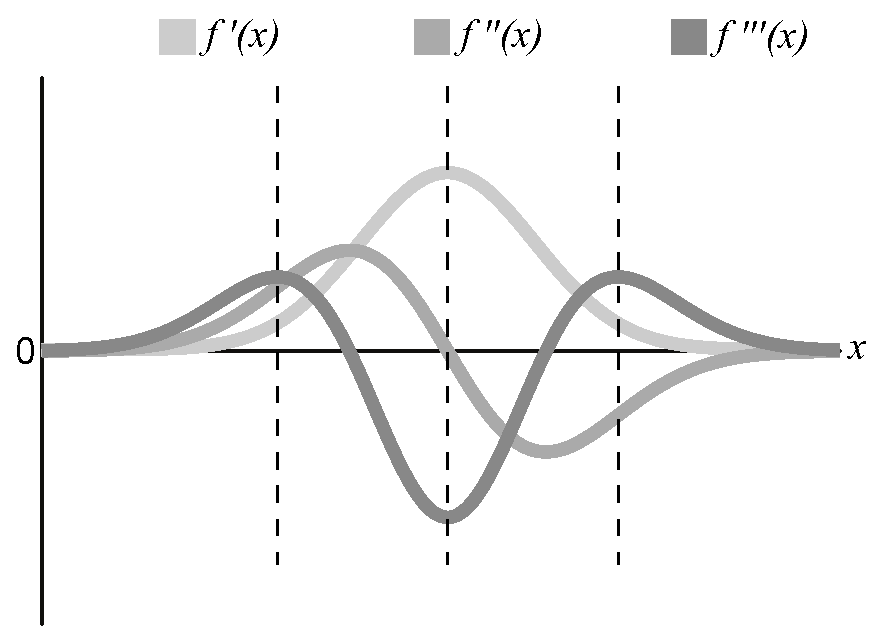
\includegraphics[width=0.7\textwidth]{images/m_inflection}
	\caption{Primeira, segunda e terceira derivadas na direção do gradiente, centradas na ocorrência de uma fronteira.}
	\label{fig:m_inflection}
\end{figure}

	No capítulo anterior foi visto que as derivadas médias $ g(v) $ e $ h(v) $ mantém os mesmos pontos característicos de $ f'(x) $ e $ f''(x) $ que identificam uma fronteira. Então, é preciso verificar que o mesmo ocorre com a terceira derivada média $ t(v) $. Para fazer tal demonstração, criou-se um volume sintético que consiste em duas esferas concêntricas, de raios e intensidades distintas, onde as fronteiras se comportam idealmente.
	
	A fatia do volume, exibida na Figura~\ref{fig:m_double_sphere}~\ref{fig:m_double_sphere_slice}, mostra que ele possui fronteiras nos intervalos $ [0,127] $ e $ [127,255] $. Portanto, espera-se que o centro das fronteiras estejam próximos a $ 64 $ e $ 190 $. Na Figura~\ref{fig:m_double_sphere}~\ref{fig:m_double_sphere_deriv} percebe-se que as derivadas médias se comportam exatamente como o esperado, pois $ 64 $ e $ 190 $ são justamente os pontos de primeira derivada máxima, segunda derivada zero e terceira derivada mínima.
	
\begin{figure}[h]
	\centering
	\subfigure[Fatia do volume]
	{
		\includegraphics[width=0.3\textwidth]{images/m_double_sphere_slice}
		\label{fig:m_double_sphere_slice}
	}
	\subfigure[Derivadas médias do volume]
	{
		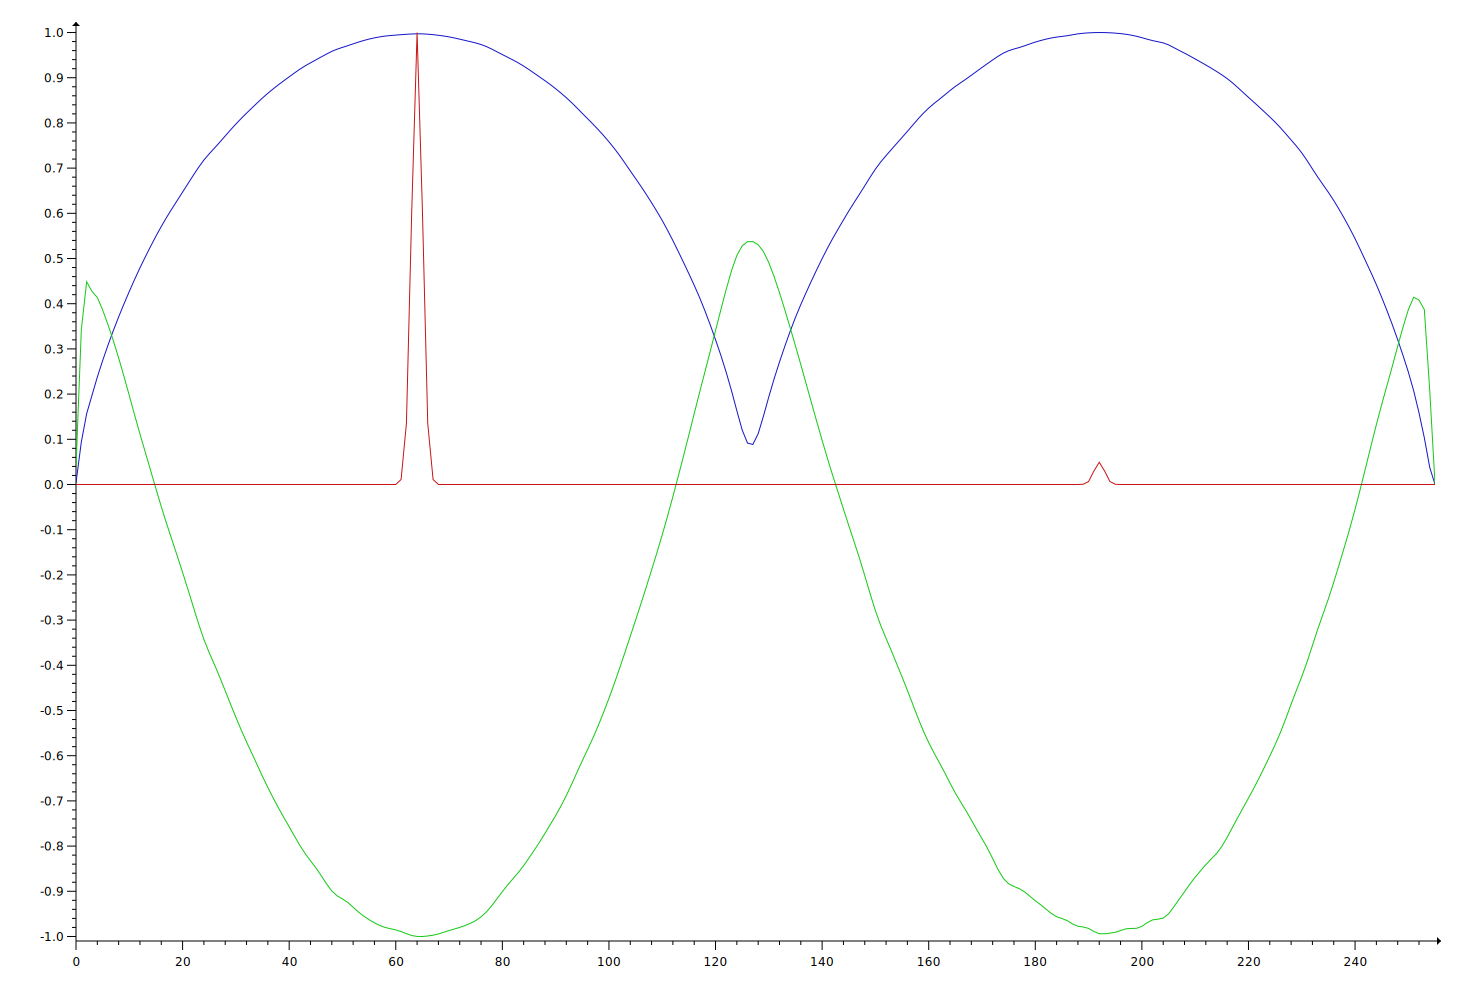
\includegraphics[width=0.6\textwidth]{images/m_double_sphere_derivatives}
		\label{fig:m_double_sphere_deriv}
	}
	\caption{Duas esferas concêntricas sem sobreposição no intervalo de valores das fronteiras.}
	\label{fig:m_double_sphere}
\end{figure}

	No entanto, $ h(v) $ é igual a zero em $ 127 $, indicando uma fronteira que não existe. Para este exemplo sintético e ideal, como o valor de $ g(v) $ é baixo, a função $ p(v) $ nesse ponto resulta em uma distância maior que a ocorrida em $ 64 $ e $ 190 $. Dessa forma, a fronteira falsa é sempre menos opaca que as fronteias reais no método de \textit{Kindlmann e Durkin}~\cite{gordon}, mas dependendo da função $ b(x) $ definida pelo usuário, a falsa fronteira pode acabar sendo realçada e visualizada, como ilustra a Figura~\ref{fig:m_double_sphere_tf}.
	
	A visualização volumétrica apresentada na Figura~\ref{fig:m_double_sphere_tf}~\ref{fig:m_double_sphere_right}, que realça corretamente as fronteiras do volume, foi obtida com a função de transferência indicada na Figura~\ref{fig:m_double_sphere_tf}~\ref{fig:m_double_sphere_tf_right}, onde utilizou-se $ b(x) $ com largura igual a $ 1 $. No entanto, ao aumentar a largura de $ b(x) $ para $ 3 $, obtém-se uma FT com um novo comportamento, ilustrada na Figura~\ref{fig:m_double_sphere_tf}~\ref{fig:m_double_sphere_tf_wrong}. Como resultado, a nova visualização apresenta uma falsa fronteira em amarelo que pode ser vista na Figura~\ref{fig:m_double_sphere_tf}~\ref{fig:m_double_sphere_wrong}.

\begin{figure}[h]
	\centering
	\subfigure[]
	{
		\includegraphics[width=0.4\textwidth]{images/m_double_sphere}
		\label{fig:m_double_sphere_right}
	}
	\subfigure[]
	{
		\includegraphics[width=0.4\textwidth]{images/m_double_sphere_wrong}
		\label{fig:m_double_sphere_wrong}
	}
	\subfigure[]
	{
		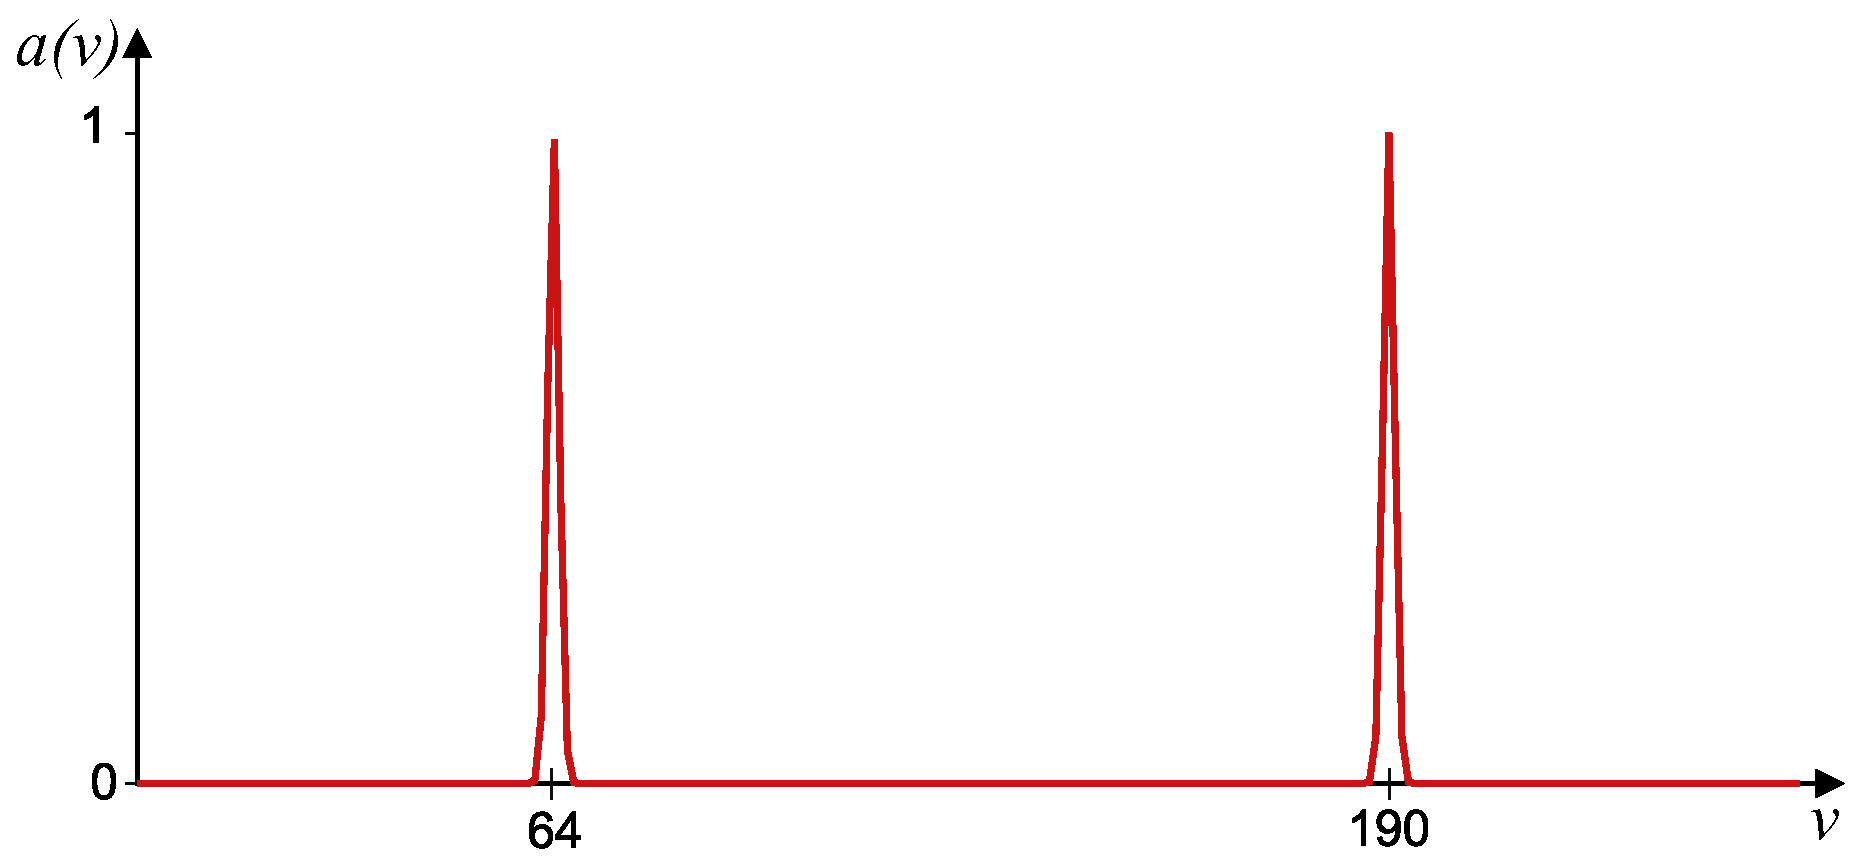
\includegraphics[width=0.7\textwidth]{images/m_double_sphere_tf_right}
		\label{fig:m_double_sphere_tf_right}
	}
	\subfigure[]
	{
		\includegraphics[width=0.7\textwidth]{images/m_double_sphere_tf_wrong}
		\label{fig:m_double_sphere_tf_wrong}
	}
	\caption{Duas esferas concêntricas sem sobreposição no intervalo de valores das fronteiras.}
	\label{fig:m_double_sphere_tf}
\end{figure}

	É preciso lembrar também que as funções $ g(v) $, $ h(v) $ e $ t(v) $ raramente apresentarão o comportamento exibido na Figura~\ref{fig:m_double_sphere}~\ref{fig:m_double_sphere_deriv}. Nos volumes em que o intervalo de valores das fronteiras se sobrepõem, a média afeta o comportamento dos arcos esperados. Para demonstrar esse fenômeno, outro volume sintético foi criado, também contendo duas esferas concêntricas, onde as fronteiras se comportam de forma ideal. Porém, neste segundo, o intervalo de valores das fronteiras se sobrepõem. A Figura~\ref{fig:m_double_sphere_disc} exibe uma fatia do volume e também suas derivadas médias.
	
	Como pode ser observado na Figura~\ref{fig:m_double_sphere_disc}~\ref{fig:m_double_sphere_disc_slice}, os intervalos das fronteiras são $ [0,255] $ e $ [170,255] $. Percebe-se que devido à sobreposição de valores, as funções não se comportam como o esperado. Apesar de existir uma fronteira entre $ 0 $ e $ 255 $, as derivadas não exibem um arco único entre esses valores. A Figura~\ref{fig:m_double_sphere_disc}~\ref{fig:m_double_sphere_disc_deriv} mostra que o arco é interrompido justamente no valor $ 170 $, que é o início da segunda fronteira e, por isso, um arco destorcido se estende até $ 255 $.	Porém, os mínimos locais em $ t(v) $ ainda são boas aproximações para o centro das fronteiras ($ 127 $ e $ 213 $).
	
\begin{figure}[h]
	\centering
	\subfigure[Fatia do volume]
	{
		\includegraphics[width=0.3\textwidth]{images/m_double_disc_sphere_slice}
		\label{fig:m_double_sphere_disc_slice}
	}
	\subfigure[Derivadas médias do volume]
	{
		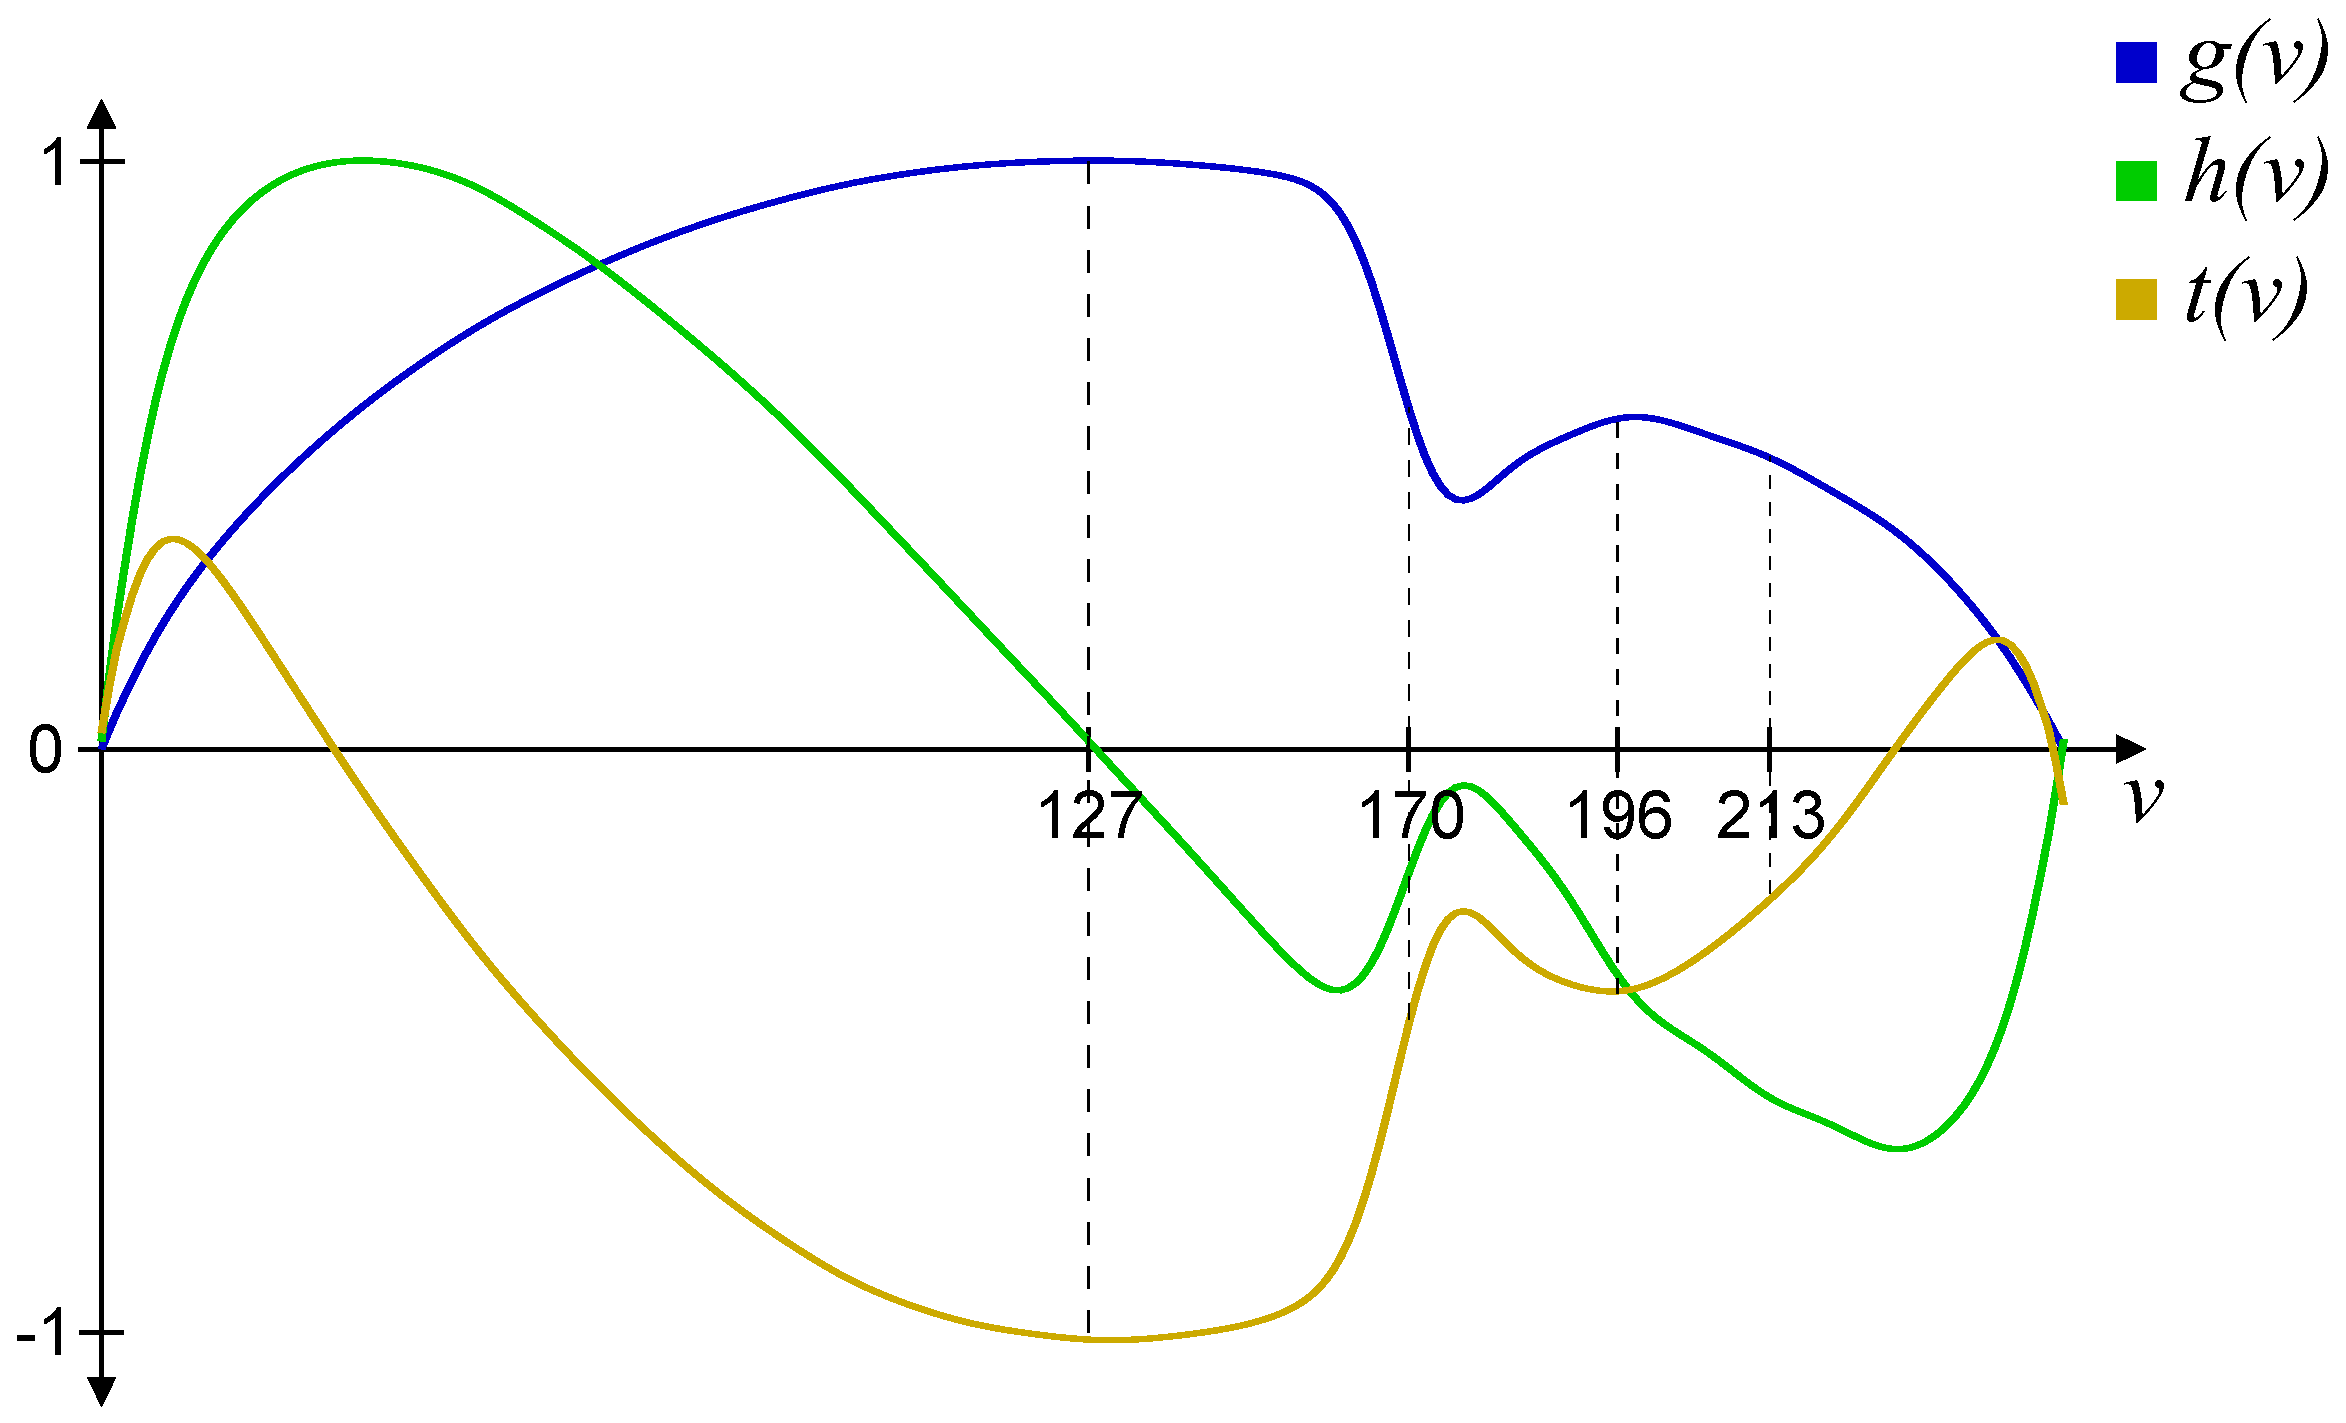
\includegraphics[width=0.6\textwidth]{images/m_double_disc_sphere_derivatives}
		\label{fig:m_double_sphere_disc_deriv}
	}
	\caption{Duas esferas concêntricas com sobreposição no intervalo de valores das fronteiras.}
	\label{fig:m_double_sphere_disc}
\end{figure}
	
	Em contra partida, a função $ h(v) $ de \textit{Kindlmann e Durkin}~\cite{gordon} identifica uma fronteira muito próxima a $ 170 $, que na verdade é a intensidade da esfera interna. Já a função $ t(v) $ apresenta uma fronteira em $ 195 $: um valor mais próximo do centro exato da fronteira (que seria $ 213 $). Então, a terceira derivada pode ser utilizada no lugar da segunda, a fim de obter funções de transferência mais precisas. Contudo, para identificar uma fronteira a partir da terceira derivada é preciso obter uma nova relação para extrair $ \sigma $ e $ x $, mas agora utilizando $ f'(x) $ e $ f'''(x) $. Para facilitar a leitura, $ f'(x) $ é repetida na Equação~\eqref{eq:first2}, enquanto a função $ f'''(x) $ é definida na Equação~\eqref{eq:third}.
	
\begin{equation} \label{eq:first2}
g = f'(x) = \frac{v_{max} - v_{min}}{\sigma\sqrt{2\pi}}\ e^{-\frac{x^{2}}{2\sigma^{2}}}
\end{equation} \

\begin{equation} \label{eq:third}
t = f'''(x) = -\frac{(x^{2} - \sigma^{2})(v_{max} - v_{min})}{\sigma^{5}\sqrt{2\pi}}\ e^{-\frac{x^{2}}{2\sigma^{2}}}
\end{equation} \
	
	Devido ao fato de $ f'(x) $ ter um grande termo em comum com $ f'''(x) $, a simples divisão entre essas funções revela uma relação envolvendo $ \sigma $ e $ x $, como mostra a Equação~\eqref{eq:sigmax}. Com $ x = 0 $ percebe-se que, mais uma vez, o valor de $ \sigma $ pode ser recuperado através dos valores extremos das derivadas, indicado na Equação~\eqref{eq:sigma3}. Por fim, $ x $ pode ser isolado na Equação~\eqref{eq:sigmax} resultando em uma nova expressão para a distância ao centro da fronteira, indicada na Equação~\eqref{eq:x3}.

\begin{equation} \label{eq:sigmax}
	\frac{f'''(x)}{f'(x)} = \frac{x^{2} - \sigma^{2}}{\sigma^{4}}
\end{equation} \

\begin{equation} \label{eq:sigma3}
	\sigma^{2} = -\frac{f'(0)}{f'''(0)} \ \approx \ -\frac{g(v)_{max}}{t(v)_{min}}
\end{equation} \

\begin{equation} \label{eq:x3}
	x = \sigma^{2}\sqrt{\frac{f'''(x)}{f'(x)} + \frac{1}{\sigma^{2}}} \ \approx \ 
	p(v) = \sigma^{2}\sqrt{\frac{t(v)}{g(v)} + \frac{1}{\sigma^{2}}}
\end{equation} \

	À primeira vista, o uso da terceira derivada no lugar da segunda garante que o deslocamento das curvas médias não resultará na atribuição de um $ v $ incorreto à fronteira. No entanto, isso ainda pode ocorrer indiretamente, a partir da distância $ x $. Uma análise da contribuição de $ \sigma $ para o valor de $ x $ ajuda a entender melhor essa relação.
	
	$ p(v) $ é igual a zero apenas quando $ \frac{t(v)}{g(v)} = -\frac{1}{\sigma^{2}} $, já que $ \sigma $ não pode ser zero. Como $ \sigma $ é obtido a partir dos valores extremos de $ g(v) $ e $ t(v) $, qualquer deslocamento nessas funções altera seu valor. Consequentemente, $ p(v) = 0 $ pode ocorrer em um $ v $ que não corresponde exatamente ao centro da fronteira. 
	
	A Figura~\ref{fig:m_sigma} ilustra como uma pequena variação no valor de $ \sigma $ pode ter um grande impacto na função de transferência. As curvas exibidas são referentes ao mesmo volume utilizado na Figura~\ref{fig:m_double_sphere}. O $ \sigma $ de valor $ 2,21 $ é o teoricamente correto, obtido através da Equação~\eqref{eq:sigma3}. A função de transferência resultante do uso deste $ \sigma $ realça muito mais a fronteira em $ 64 $ que em $ 190 $. Além disso, a FT em $ 64 $ apresenta um formato em \quote{U}, possuindo dois picos com um vale no meio onde deveria haver um só pico.
	
	Variando $ \sigma $ em apenas $ 0.02 $ vê-se que a função de transferência alterna entre realçar apenas a fronteira em $ 64 $, com baixa opacidade, e identificar as duas fronteiras apresentando um formato em \quote{U}, evidenciando que o $ \sigma $ pode provocar um deslocamento em $ p(v) $.
	
	A rigor, cada fronteira deveria possuir seu próprio sigma. De fato, durante a aquisição dos dados, o volume gerado incorpora um borrão uniforme, que ao ser representado por uma gaussiana implica em um único valor para $ \sigma $. No entanto, como diferentes fronteiras podem possuir espessuras distintas, nos casos em que o volume possui mais de uma fronteira, expressar essa espessura por um sigma único leva a uma função de transferência menos adequada.
	
	Mais estudos precisam ser feitos a fim de se distinguir a espessura de fronteiras distintas, matematicamente. Entretanto, ao invés de obter parâmetros para corrigir $ p(v) $, como \textit{Kindlmann e Durkin}~\cite{gordon} fizeram com $ g_{thresh} $, uma nova abordagem pode ser pensada para identificar fronteiras a partir dos valores extremos de $ f'(x) $ e $ f'''(x) $. Por exemplo, uma métrica pode ser desenvolvida para atribuir opacidade ao volume, baseada nos máximos e mínimos locais de $ g(v) $ e $ t(v) $.
	
\begin{figure}
	\centering
	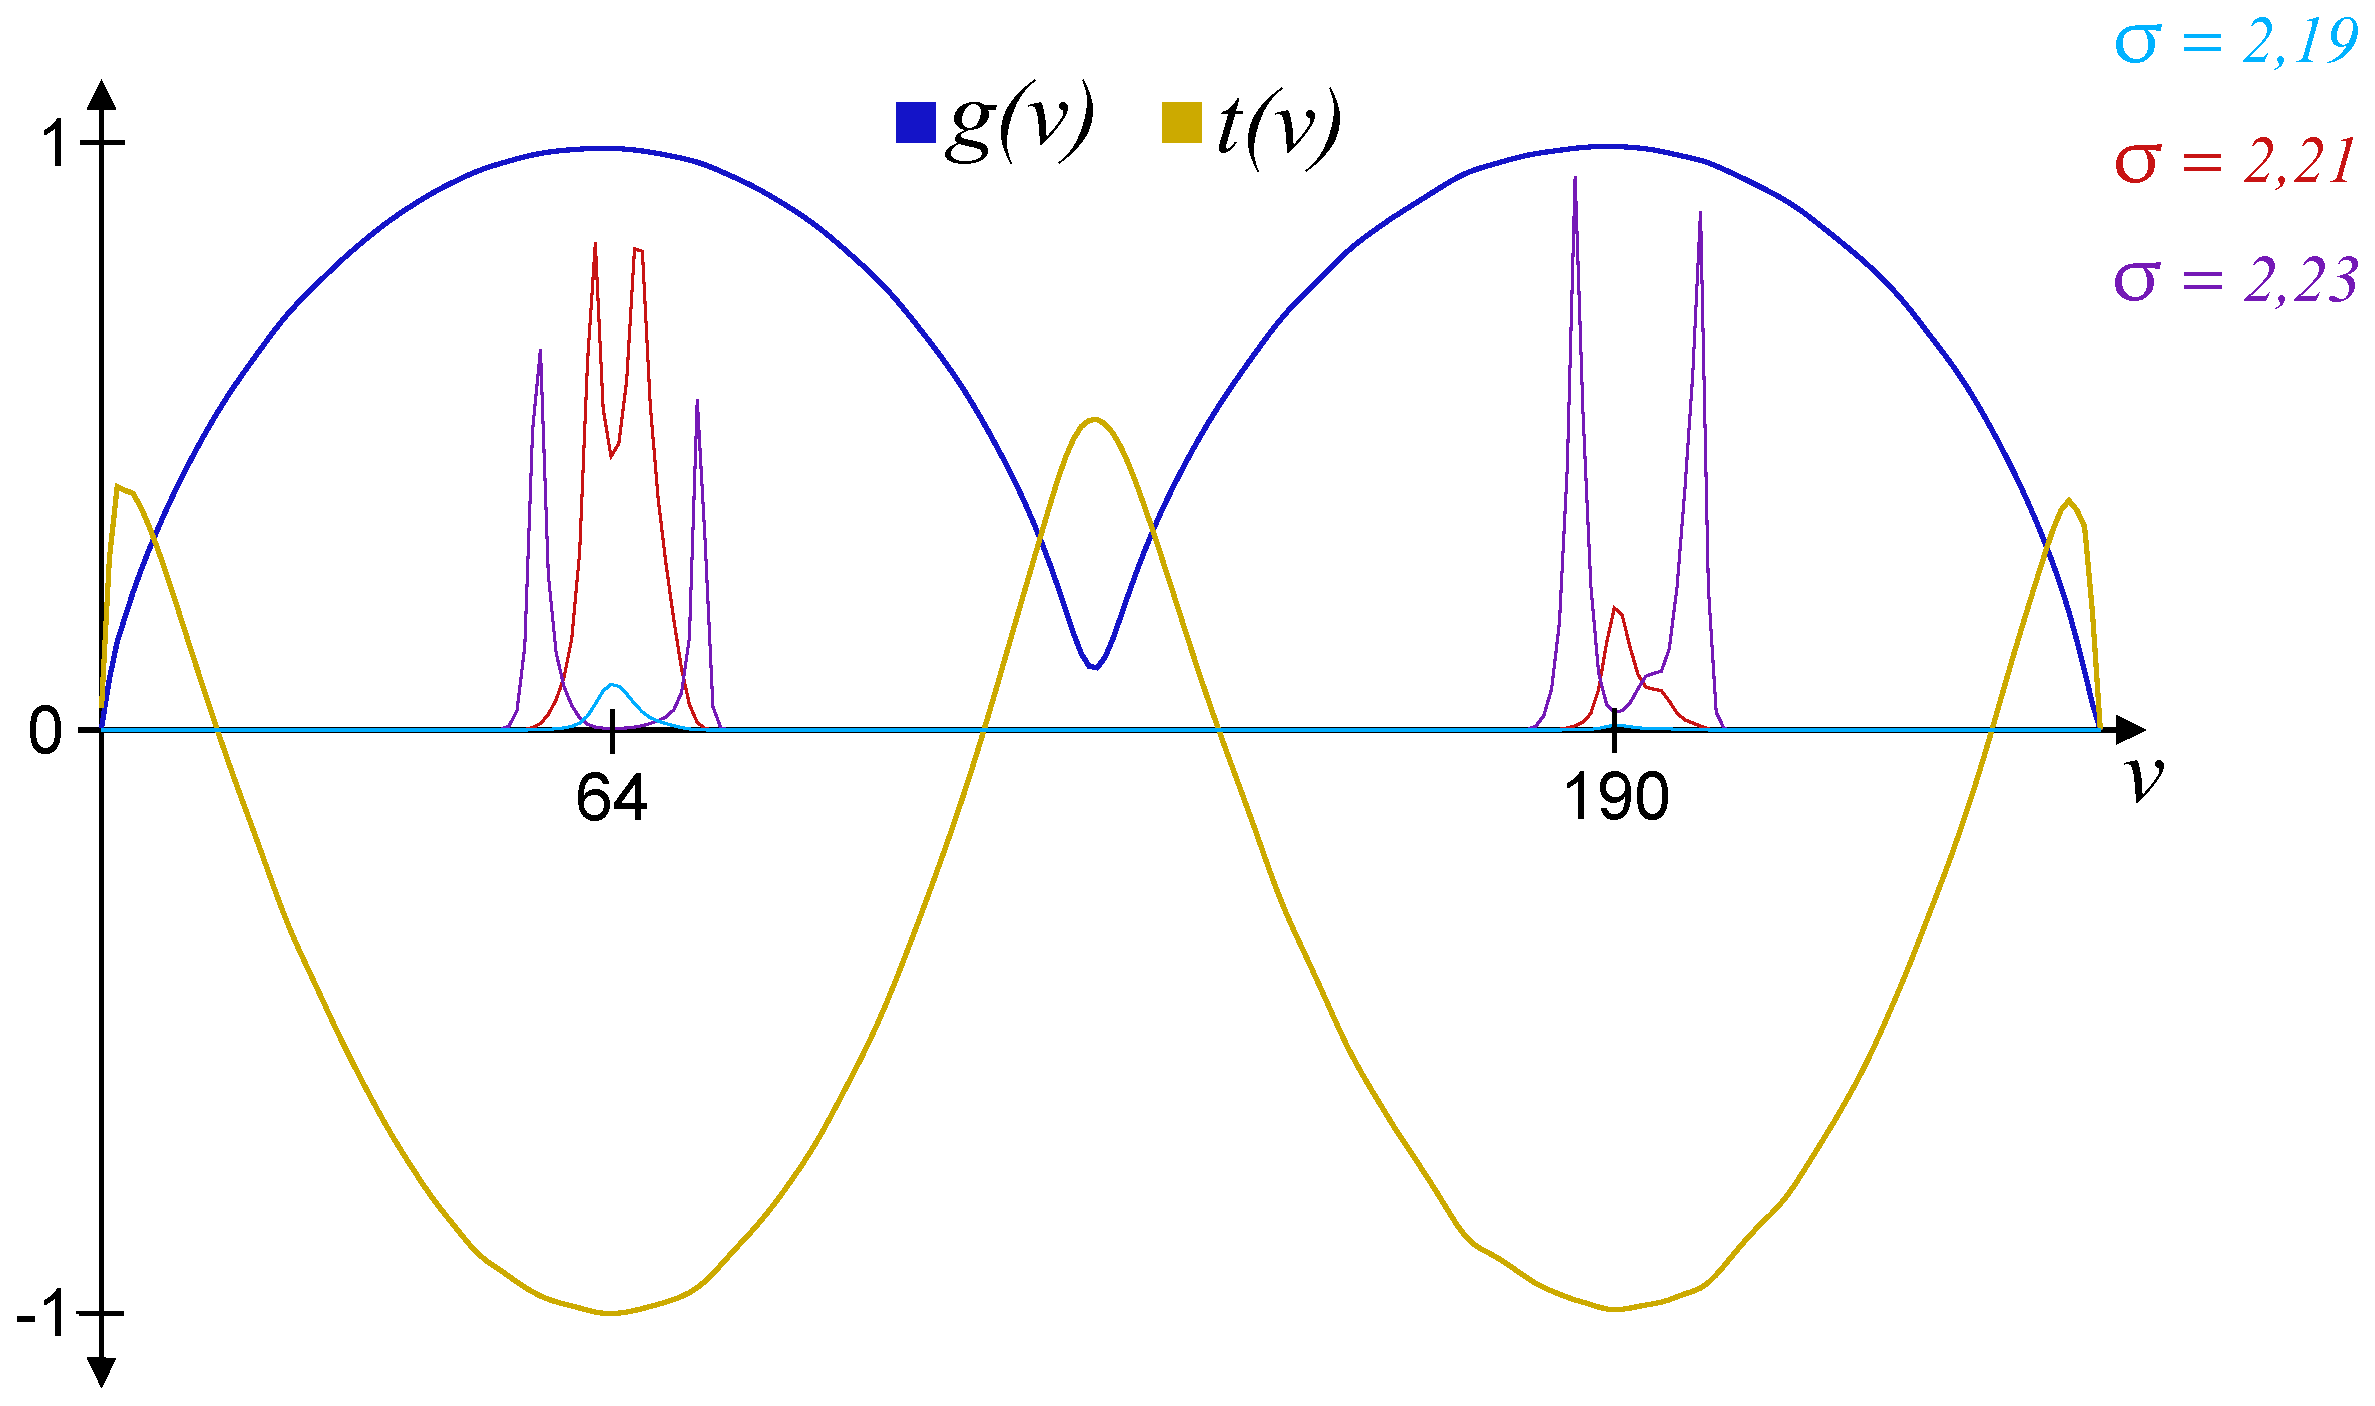
\includegraphics[width=0.7\textwidth]{images/m_sigma}
	\caption{O impacto da variação do $ \sigma $ na função de transferência.}
	\label{fig:m_sigma}
\end{figure}
	
	Como a terceira derivada é mais sensível que a primeira, ela possui uma curva mais expressiva em relação aos extremos locais. Essa característica faz com que a terceira derivada seja mais robusta em relação a falsos positivos, isto é, ela tende a apresentar menos extremos locais que não indicam uma fronteira, mas que existem em decorrência da média dos valores. Ao mesmo tempo, a terceira derivada conserva melhor seus extremos locais, não perdendo-os devido à suavização que é inerente quando se tira uma média.
	
\begin{figure}
	\centering
	\subfigure[Fatia do volume.]
	{
		\includegraphics[width=0.2\textwidth]{images/m_triple_sphere_slice}
		\label{fig:m_triple_slice}
	}
	\subfigure[Funções $ g(v) $ e $ t(v) $.]
	{
		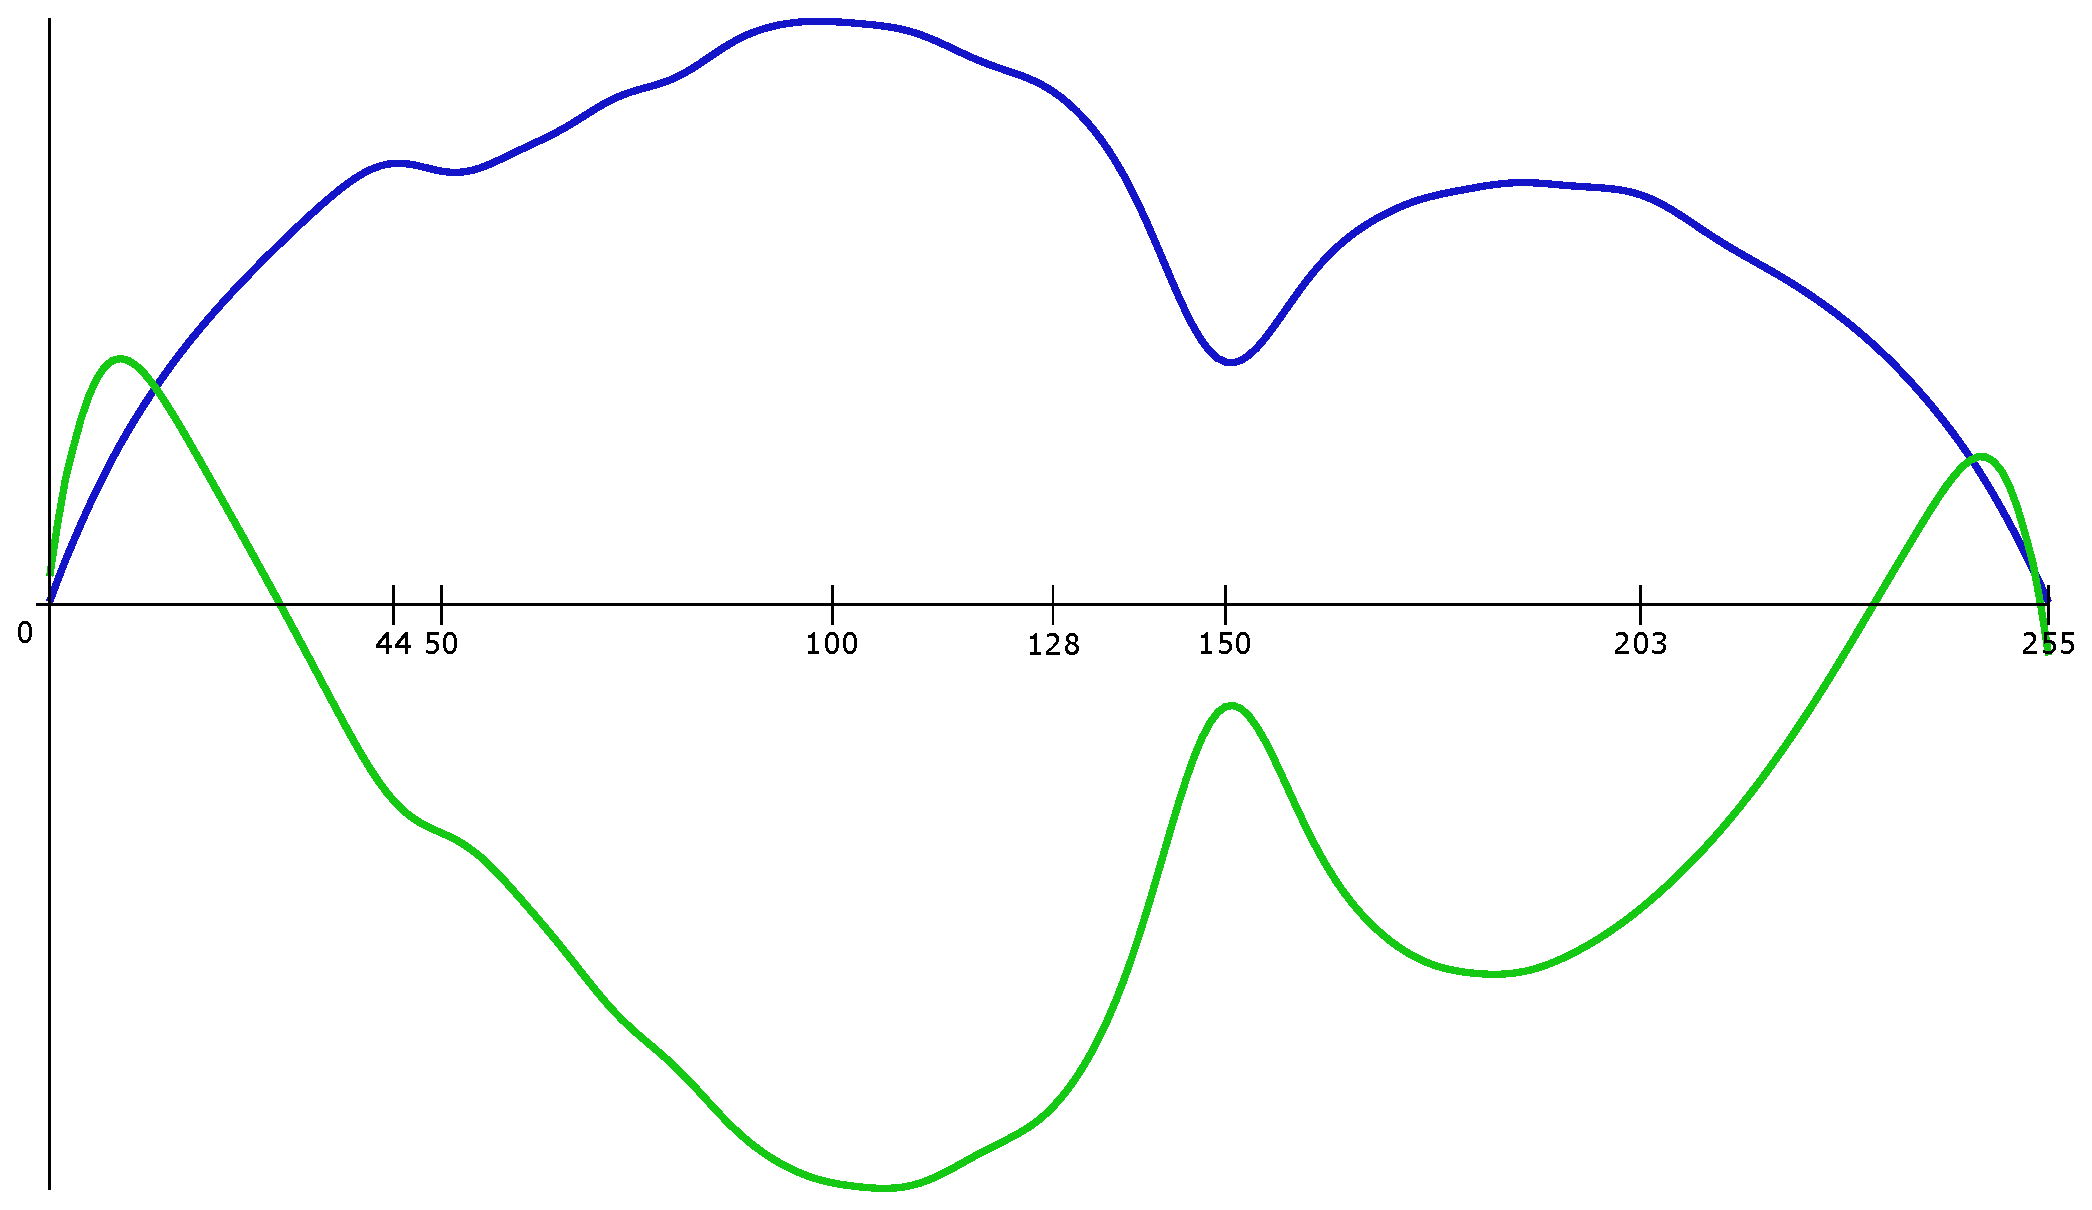
\includegraphics[width=0.7\textwidth]{images/m_triple_sphere_ft}
		\label{fig:m_triple_ft}
	}
	\caption{Volume sintético composto por três esferas concêntricas.}
	\label{fig:m_triple}
\end{figure}
	
	Um volume sintético composto por três esferas concêntricas foi utilizado para ilustrar como as derivadas médias podem exibir quantidades diferentes de extremos locais. Uma fatia do volume, exibida na Figura~\ref{fig:m_triple}~\ref{fig:m_triple_slice}, mostra que existem três fronteiras nos seguintes intervalos: $ [0,255] $, $ [50,150] $ e $ [150,255] $. Portanto, as fronteiras estão próximas a $ 128 $, $ 100 $ e $ 203 $, respectivamente. Como pode ser visto na Figura~\ref{fig:m_triple}~\ref{fig:m_triple_ft}, a primeira derivada apresenta um extremo local em $ 44 $ que não corresponde a uma fronteira. O mesmo não ocorre com a terceira derivada.
	
	Então, escolheu-se utilizar simplesmente os mínimos locais de $ t(v) $ para identificar o centro das fronteiras. Além de eliminar o $ g_{thresh} $, o resultado desta abordagem é uma função de transferência composta por um conjunto de funções de opacidade atribuídas às isosuperfícies mais importantes do volume. Essa característica permite que o usuário escolha quais fronteiras deseja visualizar. 
	
	Na Seção~\ref{sec:my.tf} a métrica exata de como gerar a função de transferência será descrita. As subseções abaixo apresentam como calcular a terceira derivada do volume de dados.
	
\subsection{Cálculo das Derivadas}
	Para calcular as derivadas é preciso lembrar que o volume não possui uma função analítica $ f(x, y, z) $ que o defina. Ele contém apenas um mapeamento de uma posição $ (x, y, z) $ para um valor escalar $ v $. Portanto, as derivadas de cada ponto do volume precisam ser calculadas com base na sua vizinhança e esse cálculo pode variar de acordo com o tipo do volume de dados.
	
	Se um volume pode ser representado por uma malha regular, então ele é espacialmente delimitado por uma caixa retangular, preenchida por células cúbicas alinhadas aos eixos da caixa, onde cada célula representa um dado do volume. Este é o caso dos volumes resultantes da maioria dos métodos de aquisição por escaneamento de uma estrutura fisiológica real, como os exames médicos. Há ainda volumes cujos dados são topologicamente estruturados, mas que não podem ser representados por uma grade regular, pois a direção da disposição dos dados varia ao longo do volume. Então, utiliza-se uma malha não regular, composta por células hexaédricos irregulares, como é o caso dos volumes resultantes das simulações de reservatórios de petróleo utilizados nesta dissertação.
	
	A diferença entre esses dois tipos de representatividade pode ser vista na Figura~\ref{fig:meshes}, onde uma versão 2D de cada malha é ilustrada. O modo de se calcular as derivadas para cada um desses casos é discutido nas subseções seguintes.
	
\begin{figure}[h]
	\centering
	\subfigure[Malha regular]
	{
		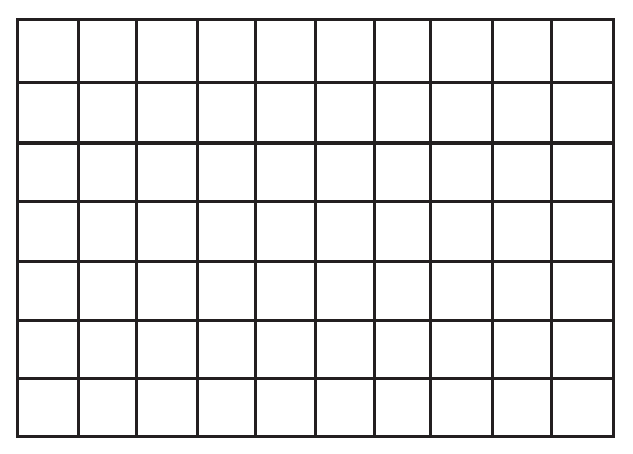
\includegraphics[width=0.3\textwidth]{images/m_regular_mesh}
	}
	\hspace{10mm}
	\subfigure[Malha não regular topologicamente estruturada]
	{
		\includegraphics[width=0.3\textwidth]{images/m_irregular_mesh}
	}
	\caption{Tipos de malhas utilizadas nesta dissertação, em 2D.}
	\label{fig:meshes}
\end{figure}
    
\subsubsection{Malhas Regulares}
\label{subsec:my.struct}

\begin{figure}[h]
	\centering
	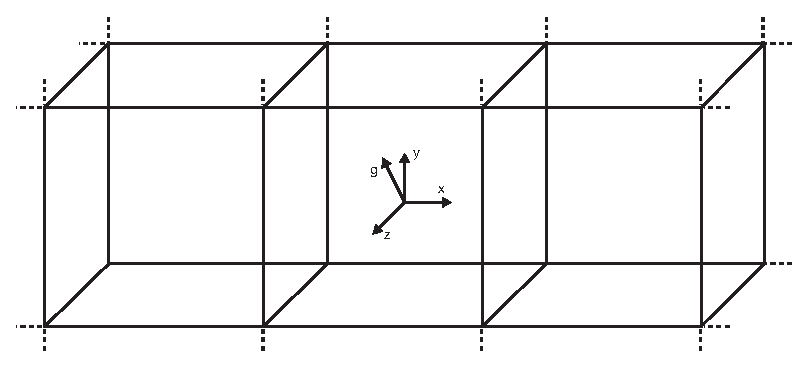
\includegraphics[width=0.7\textwidth]{images/m_regular_cells}
	\caption{Exemplo de células em malhas regulares.}
	\label{fig:m_regular_cells}
\end{figure}

	O método de diferenças finitas descreve como obter uma aproximação polinomial para a derivada de uma função $ f $ em um determinado ponto $ p $, utilizando $ n $ amostras de $ f $ equidistantes entre si a uma distância $ h $. Logo, o método das diferenças finitas pode ser utilizado para calcular as derivadas dos volumes com malhas regulares, uma vez que a distância entre suas células é sempre a mesma, na direção dos eixos.
	
	Nessa dissertação, optou-se por utilizar diferença central com $ n = 3 $. Isto é, uma das amostras é o próprio ponto $ p $ onde se deseja avaliar a derivada. As outras duas, estão a $ +h $ e $ -h $ de $ p $. A Equação~\eqref{eq:diff} mostra a primeira derivada de uma função $ f $ em um dado ponto $ p $, através de diferenças finitas centrais, como descrito acima.
	
\begin{equation}\label{eq:diff}
	f'(p) = \frac{f(p + h) - f(p - h)}{2h}
\end{equation} \

	Escolhendo o menor $ h $ discreto possível, a aplicação dessa equação no volume de dados implica em: para todas as posições do volume, computar a diferença entre os dois vizinhos mais próximos em uma mesma direção, dividido pela distância entre os mesmos. No entanto, como explicado na Seção~\ref{sec:gordon.bound}, as derivadas devem ser calculadas na direção do gradiente.
	
	O gradiente de uma função é um vetor formado pelas derivadas parciais dessa função, como indica a Equação~\eqref{eq:grad}. Assim, para cada posição do volume, o vetor gradiente também pode ser recuperado através da Equação~\eqref{eq:diff}, aproximando as derivadas nas direções $ x $, $ y $ e $ z $. Contudo, utilizar a Equação~\eqref{eq:diff} na direção do gradiente para cada posição do volume não é uma tarefa trivial, já que há apenas 3 direções do volume na qual as amostras podem ser igualmente espaçadas entre si. É preciso então recorrer à propriedade do cálculo vetorial de que a derivada direcional em uma dada direção é igual ao produto escalar do gradiente da função com o vetor da direção, como mostra a Equação~\eqref{eq:ddir}.
	
\begin{equation}\label{eq:grad}
	\nabla f = \bigg(\frac{\partial f}{\partial x}, \frac{\partial f}{\partial y}, \frac{\partial f}{\partial z}\bigg)
\end{equation} \

\begin{equation}\label{eq:ddir}
D_{\widehat{u}} f = \nabla f \cdot \widehat{u}
\end{equation} \

	Logo, a derivada na direção do gradiente é a própria norma do gradiente:

\begin{equation}\label{eq:first_derivative}
	D_{\widehat{\nabla f}} f = \nabla f \cdot \widehat{\nabla f} = \nabla f \cdot \frac{\nabla f}{\|\nabla f\|} = \|\nabla f\|
\end{equation} \

	Não é possível calcular a terceira derivada diretamente, utilizando os conceitos acima. Porém, se a magnitude do gradiente for armazenada em um novo campo escalar, a Equação~\eqref{eq:first_derivative} pode ser aplicada novamente, agora sobre $ \|\nabla f\| $. Com isso, obtém-se a segunda derivada do volume, a partir da qual pode se obter a terceira, repetindo o mesmo processo. As equações abaixo formalizam o cálculo da segunda e terceira derivadas, na direção do gradiente. 
	
	Com o fim de simplificar a compreensão das expressões, tomou-se a liberdade de representar o resultado da segunda derivada por $ \beta $.
	
\begin{align}
	\label{eq:second_derivative}
	D^{2}_{\widehat{\nabla f}} f & = D_{\widehat{\nabla f}} (\|\nabla f\|) = \nabla (\|\nabla f\|) \cdot \widehat{\nabla f} = \nabla (\|\nabla f\|) \cdot \frac{\nabla f}{\|\nabla f\|} = \beta \\
	\label{eq:third_derivative}
	D^{3}_{\widehat{\nabla f}} f & = D_{\widehat{\nabla f}} (\beta) = \nabla (\beta) \cdot \widehat{\nabla f} = \nabla (\beta) \cdot \frac{\nabla f}{\|\nabla f\|}
\end{align} \

	Antes de aplicar os conceitos discutidos até aqui, armazena-se em cada vértice a média da intensidade das células que o compartilham. Em seguida, é atribuído ao centro de cada face a média do valor dos vértices que a compõem. Dessa forma, o método de diferenças finitas é calculado entre os centros das faces de uma célula. Essa escolha faz com que o cálculo das derivadas seja igual, mesmo nas bordas do volume. Esse processo que interpola o valor escalar do centro de uma célula até o centro de suas faces é ilustrado na Figura~\ref{fig:m_cubes}.
	
\begin{figure}[h]
	\centering
	\subfigure[]
	{
		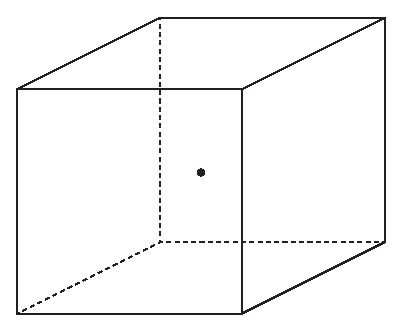
\includegraphics[width=0.3\textwidth]{images/m_cube}
	}
	\subfigure[]
	{
		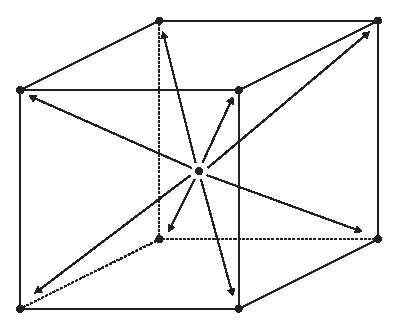
\includegraphics[width=0.3\textwidth]{images/m_cube_vertex}
	}
	\subfigure[]
	{
		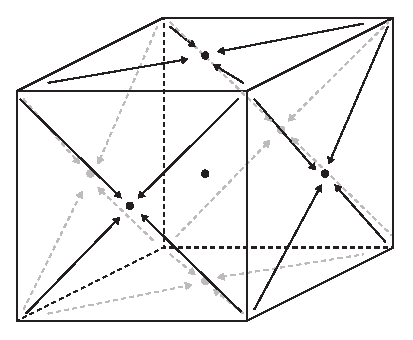
\includegraphics[width=0.3\textwidth]{images/m_cube_face}
	}
	\caption{Interpolação de valores do centro da célula para o centro das faces.}
	\label{fig:m_cubes}
\end{figure}
	
	Em posse dos valores escalares no centro das faces, a Equação~\eqref{eq:diff} é utilizada nas direções $ x $, $ y $ e $ z $, compondo respectivamente as componentes $ \frac{\partial f}{\partial x} $, $ \frac{\partial f}{\partial y} $ e $ \frac{\partial f}{\partial z} $ do gradiente $ \nabla f $. Então, a Equação~\eqref{eq:first_derivative} é aplicada e o resultado é armazenado no centro da célula, resultando no campo escalar da primeira derivada do volume. 
	
	Depois que a primeira derivada é calculada para todo o volume, a norma do gradiente armazenada no centro da célula é interpolada para o centro das faces através do mesmo processo descrito anteriormente. O vetor gradiente de cada célula já foi calculado na etapa anterior, então, pode-se aplicar a Equação~\eqref{eq:second_derivative} para obter a segunda derivada. Por fim, o resultado dessa iteração é interpolado para o centro das faces da mesma maneira, para que a terceira derivada seja calculada, de acordo com a Equação~\eqref{eq:third_derivative}.

\subsubsection{Malhas Não Regulares Topologicamente Estruturadas}
\label{subsec:my.nonstruct}

\begin{figure}[h]
	\centering
	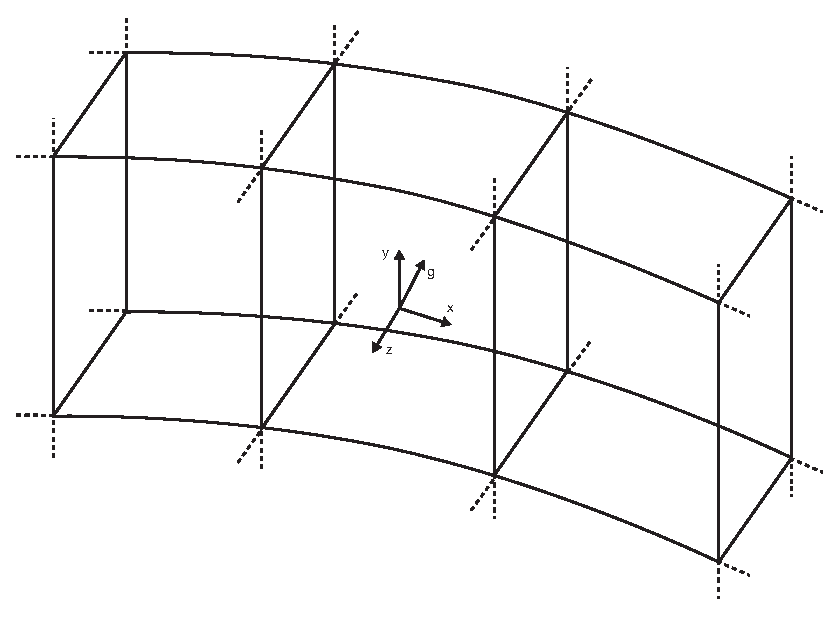
\includegraphics[width=0.7\textwidth]{images/m_irregular_cells}
	\caption{Exemplo de células em malhas não regulares topologicamente estruturadas.}
	\label{fig:m_irregular_cells}
\end{figure}

	Em malhas não regulares, a direção dos vivinhos mais próximos pode sempre variar de uma célula para outra. Portanto, a aplicação do método de diferenças finitas resultaria em derivadas direcionais distintas para cada célula, tornando inviável o uso dos conceitos apresentados até aqui. Contudo, é possível transformar o gradiente calculado no espaço paramétrico da malha, para o espaço cartesiano.
	
	Aplicando a regra da cadeia, o vetor gradiente no espaço paramétrico $ \nabla f_{(s, t, p)} $ pode ser escrito em função do vetor gradiente no espaço cartesiano $ \nabla f_{(x, y, z)} $, como mostra a Equação~\eqref{eq:cadeia}. As derivadas parciais que relacionam os dois vetores, equivalem aos termos da matriz Jacobiana do espaço paramétrico. Então, a transformação entre os espaços pode ser expressa de forma reduzida pela Equação~\eqref{eq:cadeia_jacob}.
	\\
	
\begin{equation}\label{eq:cadeia}
	\nabla f_{(s, t, p)} = \left(
	\begin{array}{ccc}
		\vspace{1mm} \frac{\partial f}{\partial s} \\
		\vspace{1mm} \frac{\partial f}{\partial t} \\
		\frac{\partial f}{\partial p}
	\end{array}
	\right)
	 = \left(
	\begin{array}{ccc}
		\vspace{1mm}
		\frac{\partial f}{\partial x}\frac{\partial x}{\partial s} + \frac{\partial f}{\partial y}\frac{\partial y}{\partial s} + \frac{\partial f}{\partial z}\frac{\partial z}{\partial s}
		\\
		\vspace{1mm}
		\frac{\partial f}{\partial x}\frac{\partial x}{\partial t} + \frac{\partial f}{\partial y}\frac{\partial y}{\partial t} + \frac{\partial f}{\partial z}\frac{\partial z}{\partial t}
		\\
		\frac{\partial f}{\partial x}\frac{\partial x}{\partial p} + \frac{\partial f}{\partial y}\frac{\partial y}{\partial p} + \frac{\partial f}{\partial z}\frac{\partial z}{\partial p}
	\end{array}
	\right)
\end{equation} \

\begin{equation}\label{eq:jacob}
	J = 
	\begin{bmatrix}
	\frac{\partial x}{\partial s} && \frac{\partial y}{\partial s} && \frac{\partial z}{\partial s} \\
	\frac{\partial x}{\partial t} && \frac{\partial y}{\partial t} && \frac{\partial z}{\partial t} \\
	\frac{\partial x}{\partial p} && \frac{\partial y}{\partial p} && \frac{\partial z}{\partial p}
	\end{bmatrix}
\end{equation} \

\begin{equation}\label{eq:cadeia_jacob}
	\nabla f_{(s, t, p)} = J\ \nabla f_{(x, y, z)}
\end{equation} \

	De forma análoga, multiplicando a equação acima pela matriz Jacobiana inversa obtém-se:
	
\begin{equation}\label{eq:cadeia_jacob_inv}
	\nabla f_{(x, y, z)} = J^{-1}\ \nabla f_{(s, t, p)}
\end{equation} \

	A matriz Jacobiana e sua inversa devem ser calculadas para o centro $ C_{i, j, k} $ de cada célula. Abaixo, $ J $ é reescrita em função dos centros das faces, onde $ C_{i + \frac{1}{2}, j, k} $ indica o centro da face entre $ C_{i, j, k} $ e $ C_{i + 1, j, k} $.

\begin{equation}\label{eq:jacob_cell}
	J = 
\begin{bmatrix}
	C_{i + \frac{1}{2}, j, k} - C_{i - \frac{1}{2}, j, k}\\
	C_{i, j + \frac{1}{2}, k} - C_{i, j - \frac{1}{2}, k}\\
	C_{i, j, k + \frac{1}{2}} - C_{i, j, k - \frac{1}{2}}
\end{bmatrix}	
\end{equation} \

	Uma vez transformado para o espaço cartesiano, o vetor gradiente pode ser armazenado na célula. Então, o mesmo processo descrito na seção anterior ocorre: a magnitude do gradiente é interpolada até o centro das faces para que a próxima derivada possa ser calculada. Para obter a segunda e terceira derivadas, transforma-se para o espaço cartesiano o gradiente do campo escalar correspondente à derivada de menor ordem. Abaixo, as expressões para a primeira, segunda e terceira derivadas são reescritas com a correção para o espaço cartesiano:
	
\begin{equation}\label{eq:derivatives_cart}
\begin{aligned}
	\vspace{4mm}
	D_{\widehat{\nabla f}} f_{(x,y,z)} & = 
		J^{-1}\ \nabla f_{(s,t,p)} 
		\cdot 
		J^{-1}\ \widehat{\nabla f}_{(s,t,p)}
		= \|\nabla f_{(x,y,z)}\|
		\\
	\vspace{4mm}
	D^{2}_{\widehat{\nabla f}} f_{(x,y,z)} & = 
		J^{-1}\ \nabla (\|\nabla f_{(x,y,z)}\|)_{(s,t,p)}
		\cdot
		J^{-1}\ \widehat{\nabla f}_{(s,t,p)}
		= \beta
		\\
	D^{3}_{\widehat{\nabla f}} f_{(x,y,z)} & = 
	J^{-1}\ \nabla (\beta)_{(s,t,p)}
	\cdot
	J^{-1}\ \widehat{\nabla f}_{(s,t,p)}
\end{aligned}
\end{equation}

\section{Geração da função de transferência}
\label{sec:my.tf}
	Após calcular as derivadas para todas as células do volume, obtém-se a média da terceira derivada para cada $ v $ (já quantizado) do volume, dando origem a $ t(v) $. Essa função naturalmente possui um perfil serrilhado, uma vez que ela é formada pela média de valores quantizados. Então, convolui-se $ t(v) $ com uma gaussiana, para suavizá-la. Por fim, a função é normalizada, dividindo-a pelo seu maior valor absoluto.
	
	Como discutido anteriormente, os mínimos locais em $ t(v) $ indicam fronteiras a serem realçadas. Portanto, todo centro de fronteira é determinado por um valor $ v_{f} $ tal que $t(v_{f}) < t(v_{f} - 1)$ e $ t(v_{f}) < t(v_{f} + 1)$. A contribuição de uma fronteira para a função de transferência é dada por uma gaussiana cuja amplitude máxima é $ |t(v_{f})| $. A espessura da gaussiana, aproximada por $ 2\sigma $, é um parâmetro que pode ser controlado pelo usuário e é inicializado com $ 2 $.
	
	Um fator de opacidade máximo $ \alpha_{max} $ foi definido para controlar melhor a transparência final da visualização. Dessa forma, o usuário possui um controle fino sobre a função de transferência, semelhante à função $ b(x) $ de \textit{Kindlmann e Durkin}~\cite{gordon}, porém, esse controle está implícito no modelo da função de transferência através de $ \sigma $ e $ \alpha_{max} $, como mostra a Equação~\eqref{eq:ft}.

\begin{equation} \label{eq:ft}
	\alpha(v) = \alpha_{max}\max_{\forall v_{f}}\big\{|t(v_{f})|e^{-\frac{(v-v_{f})^{2}}{2\sigma^{2}}}\big\}
\end{equation}\

	A equação matemática da função de transferência evidencia que ela é composta por um conjunto de gaussianas, uma para cada centro de fronteira identificado. Assim, ao substituir o termo $ \forall v_{f} $ por um conjunto de isosuperfícies contido no universo de todas as fronteiras identificadas, o usuário ganha também um controle para visualizar fronteiras de forma independente. Então, uma interface foi desenvolvida para permitir ao usuário visualizar o volume utilizando a FT gerada automaticamente, bem como realizar nela esses pequenos ajustes discutidos. 
	
	A Figura~\ref{fig:m_interface}~\ref{fig:m_interface_methods} mostra que a interface permite também alternar entre os seguintes métodos para geração automática de FTs:
	\begin{itemize}
		\item \quote{Our Method} $ \rightarrow $ Método proposto por esta dissertação.
		\item \quote{KD Method} $ \rightarrow $ Método 1D de \textit{Kindlmann e Durkin}~\cite{gordon}.
	\end{itemize}
	
	Caso o primeiro método seja selecionado, o usuário pode escolher quais fronteiras deseja visualizar. Para isso, sempre que um novo modelo é carregado, o componente exibido na Figura~\ref{fig:m_interface}~\ref{fig:m_interface_iso} é recarregado com uma lista de valores do volume nos quais há ocorrência de fronteira. Então, o usuário pode alternar entre visualizar todas (\quote{Select all}), nenhuma (\quote{Select None}), ou um conjunto específico a partir da lista apresentada.
	
	É possível ainda alternar para o modo de isovolume. Nele apenas um valor de intensidade pode ser escolhido na lista, pois a função de transferência será máxima em todos os valores superiores ao escolhido (\quote{+ IsoVolume +}), ou inferiores (\quote{- IsoVolume -}). Contudo, se o método selecionado não for o proposto por essa dissertação, as opções discutidas são desabilitadas.
	
	A Figura~\ref{fig:m_interface}~\ref{fig:m_interface_bx} mostra componentes da interface que estão sempre disponíveis, independentemente do método selecionado. Para os métodos baseados no trabalho de \textit{Kindlmann e Durkin}~\cite{gordon}, esses controles definem a própria função $ b(x) $, onde \quote{Thickness} define a largura da função gaussiana enquanto sua altura é definida pela multiplicação de \quote{Opacity Factor} e \quote{Alpha}. Caso a função de transferência utilizada seja a definida pelo método proposto, o parâmetro $ \alpha_{max} $ é obtido através do produto de \quote{Opacity Factor} com \quote{Alpha} e $ \sigma $ recebe o valor de \quote{Thickness}.% O controle \quote{Thickness} varia de $ 0,1 $ a $ 30 $ enquanto \quote{Alpha} varia de $ 0,001 $ a  $ 0,1 $.
	
\begin{figure}[H]
	\centering
	\begin{tabular}{cc}
		\begin{tabular}{c}
			\subfigure[]
			{
				\includegraphics[width=0.21\textwidth]{images/m_interface_methods}
				\label{fig:m_interface_methods}
			}\\
			\subfigure[]
			{
				\includegraphics[width=0.21\textwidth]{images/m_interface_iso}
				\label{fig:m_interface_iso}
			}
		\end{tabular}
		&
		\begin{tabular}{c}
			\subfigure[]
			{
				\includegraphics[width=0.2\textwidth]{images/m_interface_bx}
				\label{fig:m_interface_bx}
			}
		\end{tabular}
	\end{tabular}
	\caption{Campos da interface de controle do usuário.}
	\label{fig:m_interface}
\end{figure}

	Os controles da Figura~\ref{fig:m_interface} são referentes à função de transferência exibida na Figura~\ref{fig:m_interface_all}~\ref{fig:m_interface_all_tf}, cuja visualização do volume pode ser vista na Figura~\ref{fig:m_interface_all}~\ref{fig:m_interface_all_res}. Supondo uma interação do usuário com a interface, ainda sobre o mesmo volume, caso apenas a opção \quote{IsoValue 85} fosse marcada e o usuário aumentasse a largura da FT, o resultado seria a Figura~\ref{fig:m_interface_isoval}~\ref{fig:m_interface_iso_tf}. A visualização volumétrica correspondente ao uso dessa FT é exibida na Figura~\ref{fig:m_interface_isoval}~\ref{fig:m_interface_iso_res}.
	
\begin{figure}[h]
	\centering
	\subfigure[]
	{
		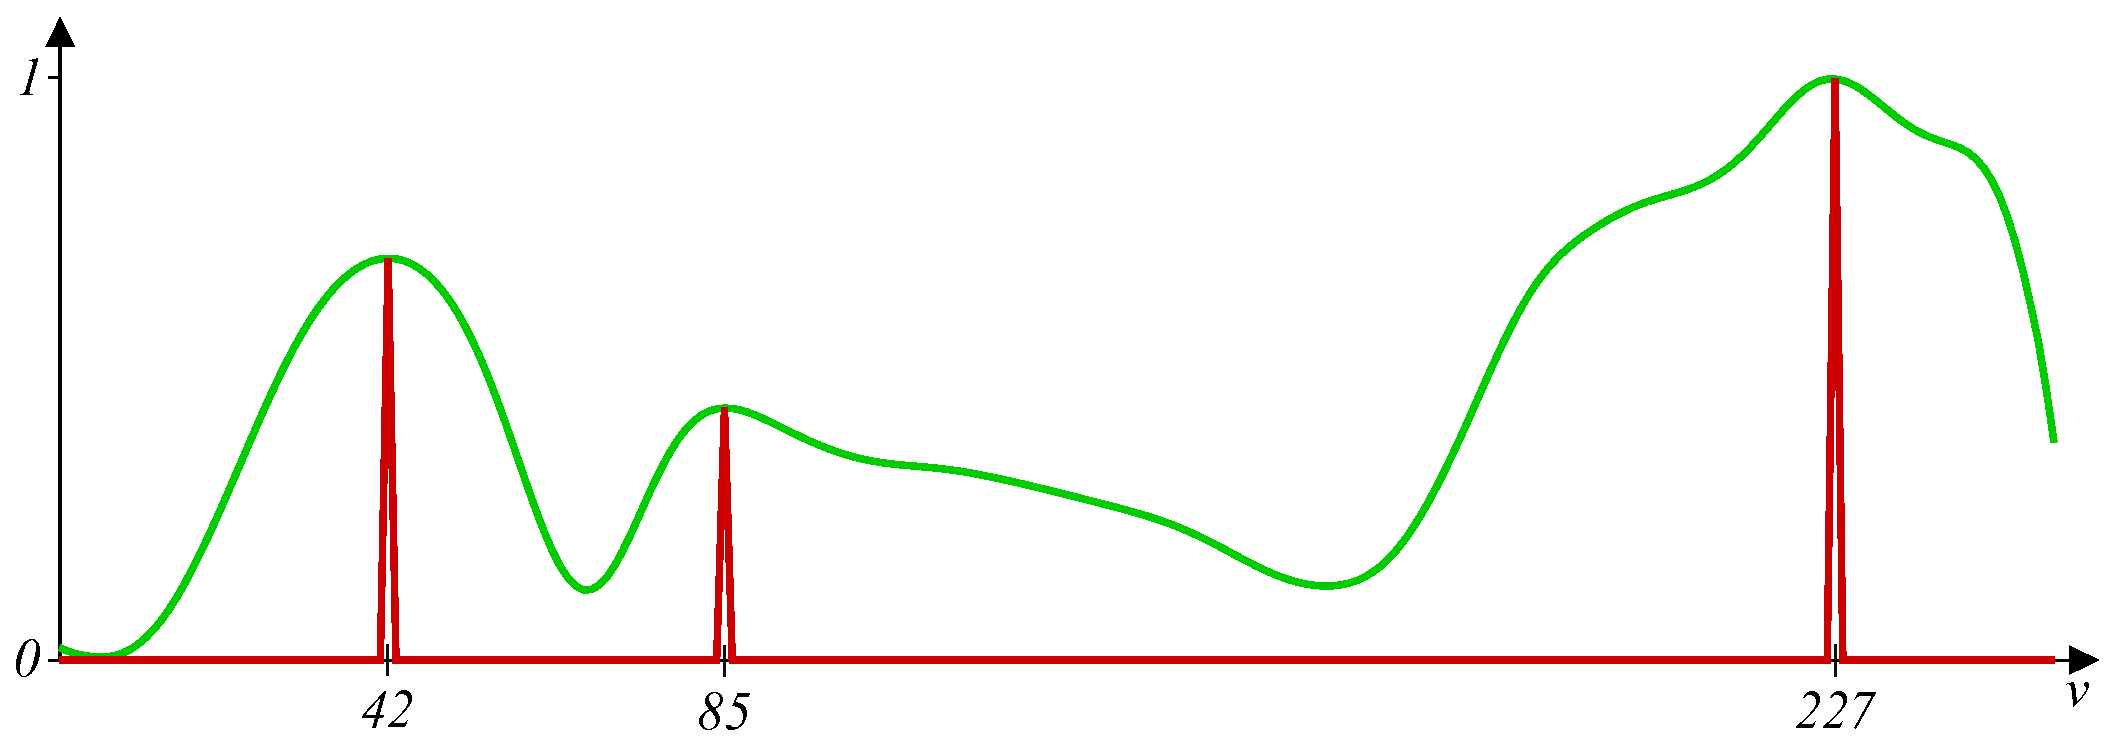
\includegraphics[width=1\textwidth]{images/m_interface_all}
		\label{fig:m_interface_all_tf}
	}
	\subfigure[]
	{
		\includegraphics[width=1\textwidth]{images/m_interface_all_res}
		\label{fig:m_interface_all_res}
	}
	\caption{}
	\label{fig:m_interface_all}
\end{figure}

\begin{figure}[h]
	\centering
	\subfigure[]
	{
		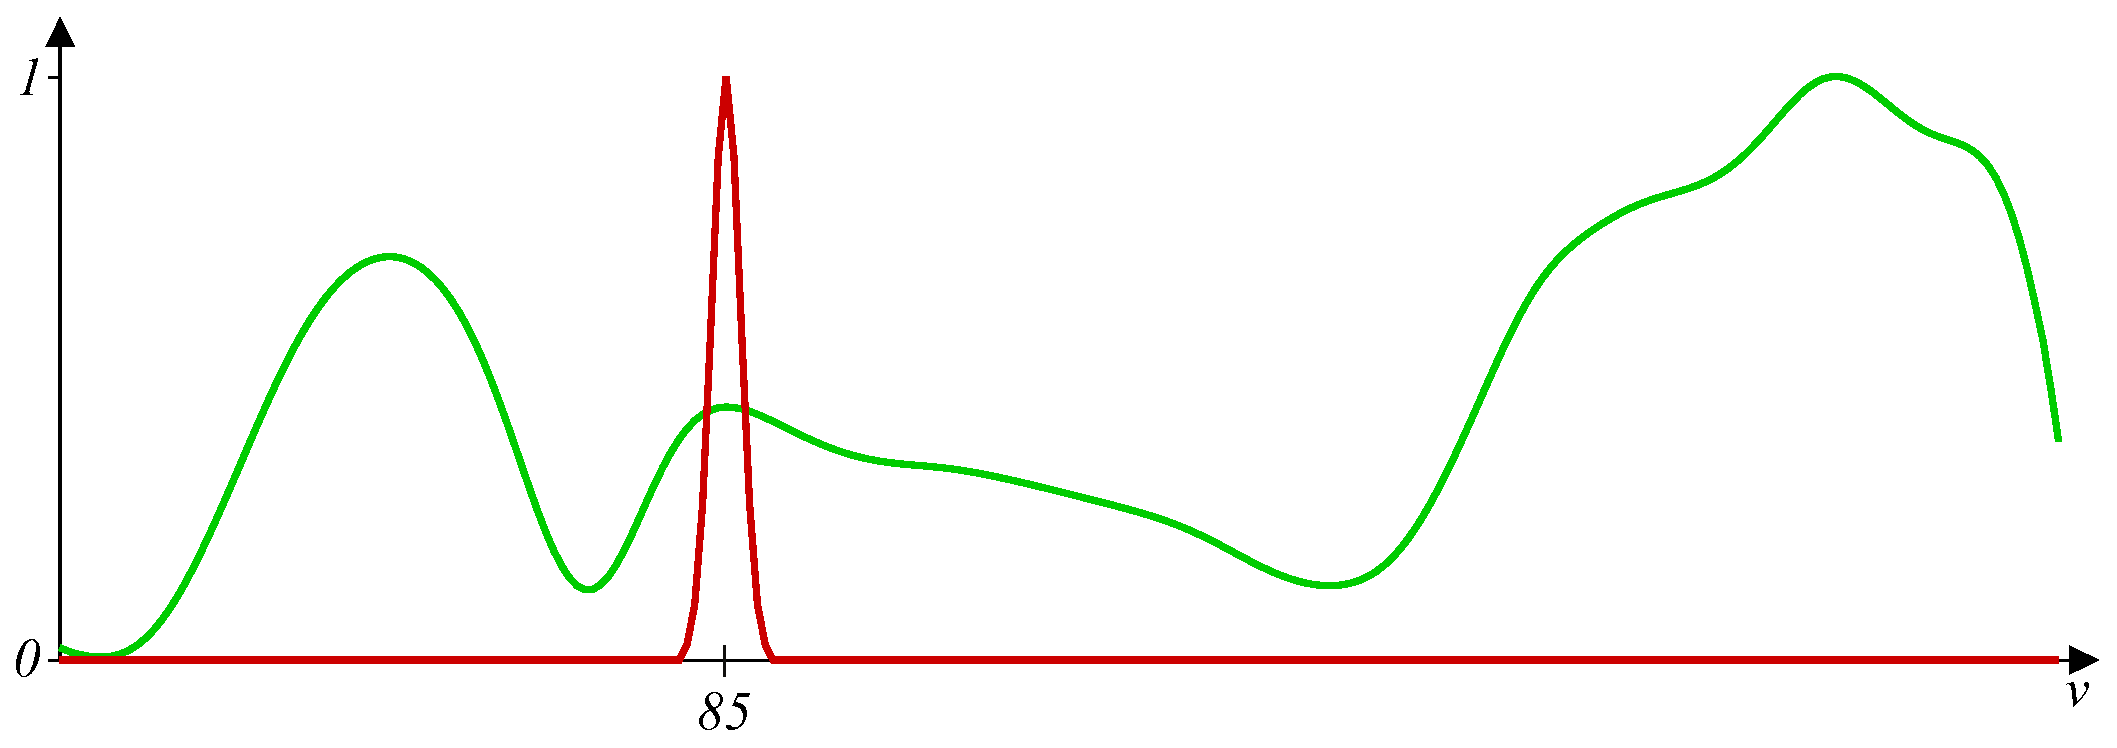
\includegraphics[width=1\textwidth]{images/m_interface_iso_tf}
		\label{fig:m_interface_iso_tf}
	}
	\subfigure[]
	{
		\includegraphics[width=1\textwidth]{images/m_interface_iso_res}
		\label{fig:m_interface_iso_res}
	}
	\caption{}
	\label{fig:m_interface_isoval}
\end{figure}
% -*- coding: utf-8; -*-

\chapter{Resultados}
\label{ch:result}

	Este capítulo apresenta os resultados desta dissertação para volumes de malhas regulares conhecidos na literatura e modelos de simulação de reservatório de petróleo, respectivamente nas Seções~\ref{sec:result.reg}~e~\ref{sec:result.irreg}. Esses resultados serão comparados com os obtidos através da aplicação do método de \textit{Kindlmann e Durkin}~\cite{gordon}. Para os volumes não regulares, oriundos de simulações de reservatório de petróleo, as derivadas são calculadas de acordo com a Subseção~\ref{subsec:my.nonstruct}.
	
	É preciso lembrar, contudo, que existem diversas técnicas de visualização volumétrica. Então, a análise feita será sempre em cima da função de transferência obtida e como esta foi capaz, ou não, de realçar as fronteiras do volume.
	
	A fim de facilitar a análise dos volumes e suas respectivas funções de transferência geradas pelos dois métodos, utilizou-se uma só escala de cores para todos os volumes, exibida na figura abaixo. O acesso à textura da escala é feito por $ v $, de forma que o primeiro texel é dado por $ v = 0 $ e o último por $ v = 255 $.

\begin{figure}[h]
	\centering
	\includegraphics[width=0.9\textwidth]{images/r_colorscale}
	\caption{Escala de cores das funções de transferência.}
\end{figure}
	
\section{Malhas Regulares}
\label{sec:result.reg}

	Para visualizar os volumes de malhas regulares utilizou-se o visualizador volumétrico apresentado por \textit{Campagnolo et al.}~\cite{lqc}, aplicando o modelo de iluminação de Blinn-Phong e a estratégia \quote{front-to-back composition}, ambos explicados no Capítulo 39 de~\cite{gems}.

%%%%%%%%%%%%%%%%%%%%%%%%%%%%%%%%%% SPHERES %%%%%%%%%%%%%%%%%%%%%%%%%%%%%%%%%%%%%
	A Figura~\ref{fig:r_sphere_slice} exibe uma fatia de um volume sintético com ruido que possui cinco fronteiras próximas aos valores $ 93 $, $ 164 $, $ 178 $, $ 192 $ e $ 210 $. Como pode ser observado na Figura~\ref{fig:r_3sphere}, o método de \textit{Kindlmann e Durkin} identifica duas fronteiras ($ 92 $ e $ 174 $), enquanto o método proposto nesta dissertação identifica quatro ($ 93 $, $ 178 $, $ 203 $ e $ 233 $). A Figura~\ref{fig:r_3sphere}~\ref{fig:r_3sphere_kd} mostra ainda que há dois pontos de máximo local na primeira derivada média (em azul) que não são realçados como fronteira, pois a segunda derivada média nesses pontos não é próxima de zero. Estes mesmos dois picos, descartados pelo método de \textit{Kindlmann e Durkin} coincidem exatamente com as duas fronteiras destacadas a mais pelo método aqui proposto, como mostra a Figura~\ref{fig:r_3sphere}~\ref{fig:r_3sphere_mine}.
	
\begin{figure}[h]
	\centering
	\includegraphics[width=0.47\textwidth]{images/r_3sphere_slice}
	\caption{Fatia do volume \quote{Test Spheres}.}
	\label{fig:r_sphere_slice}
\end{figure}

\begin{figure}[h]
	\centering
	\subfigure[Método de \textit{Kindlmann e Durkin}.]
	{
		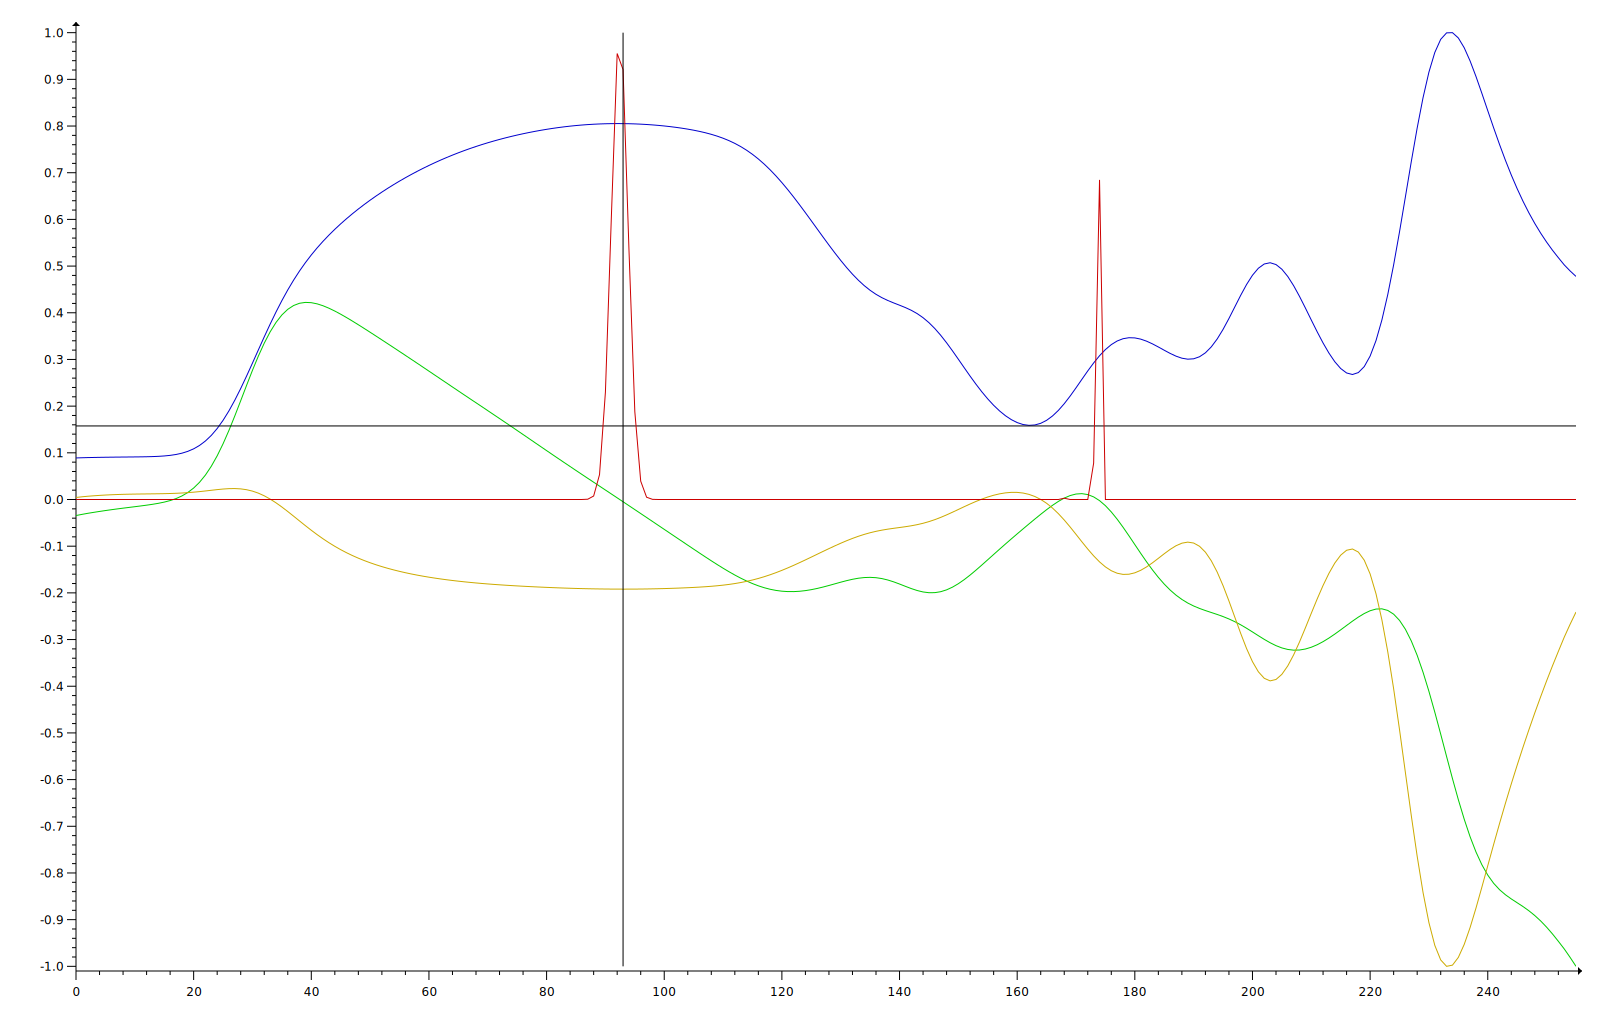
\includegraphics[width=0.35\textwidth]{images/r_g_3sphere}
		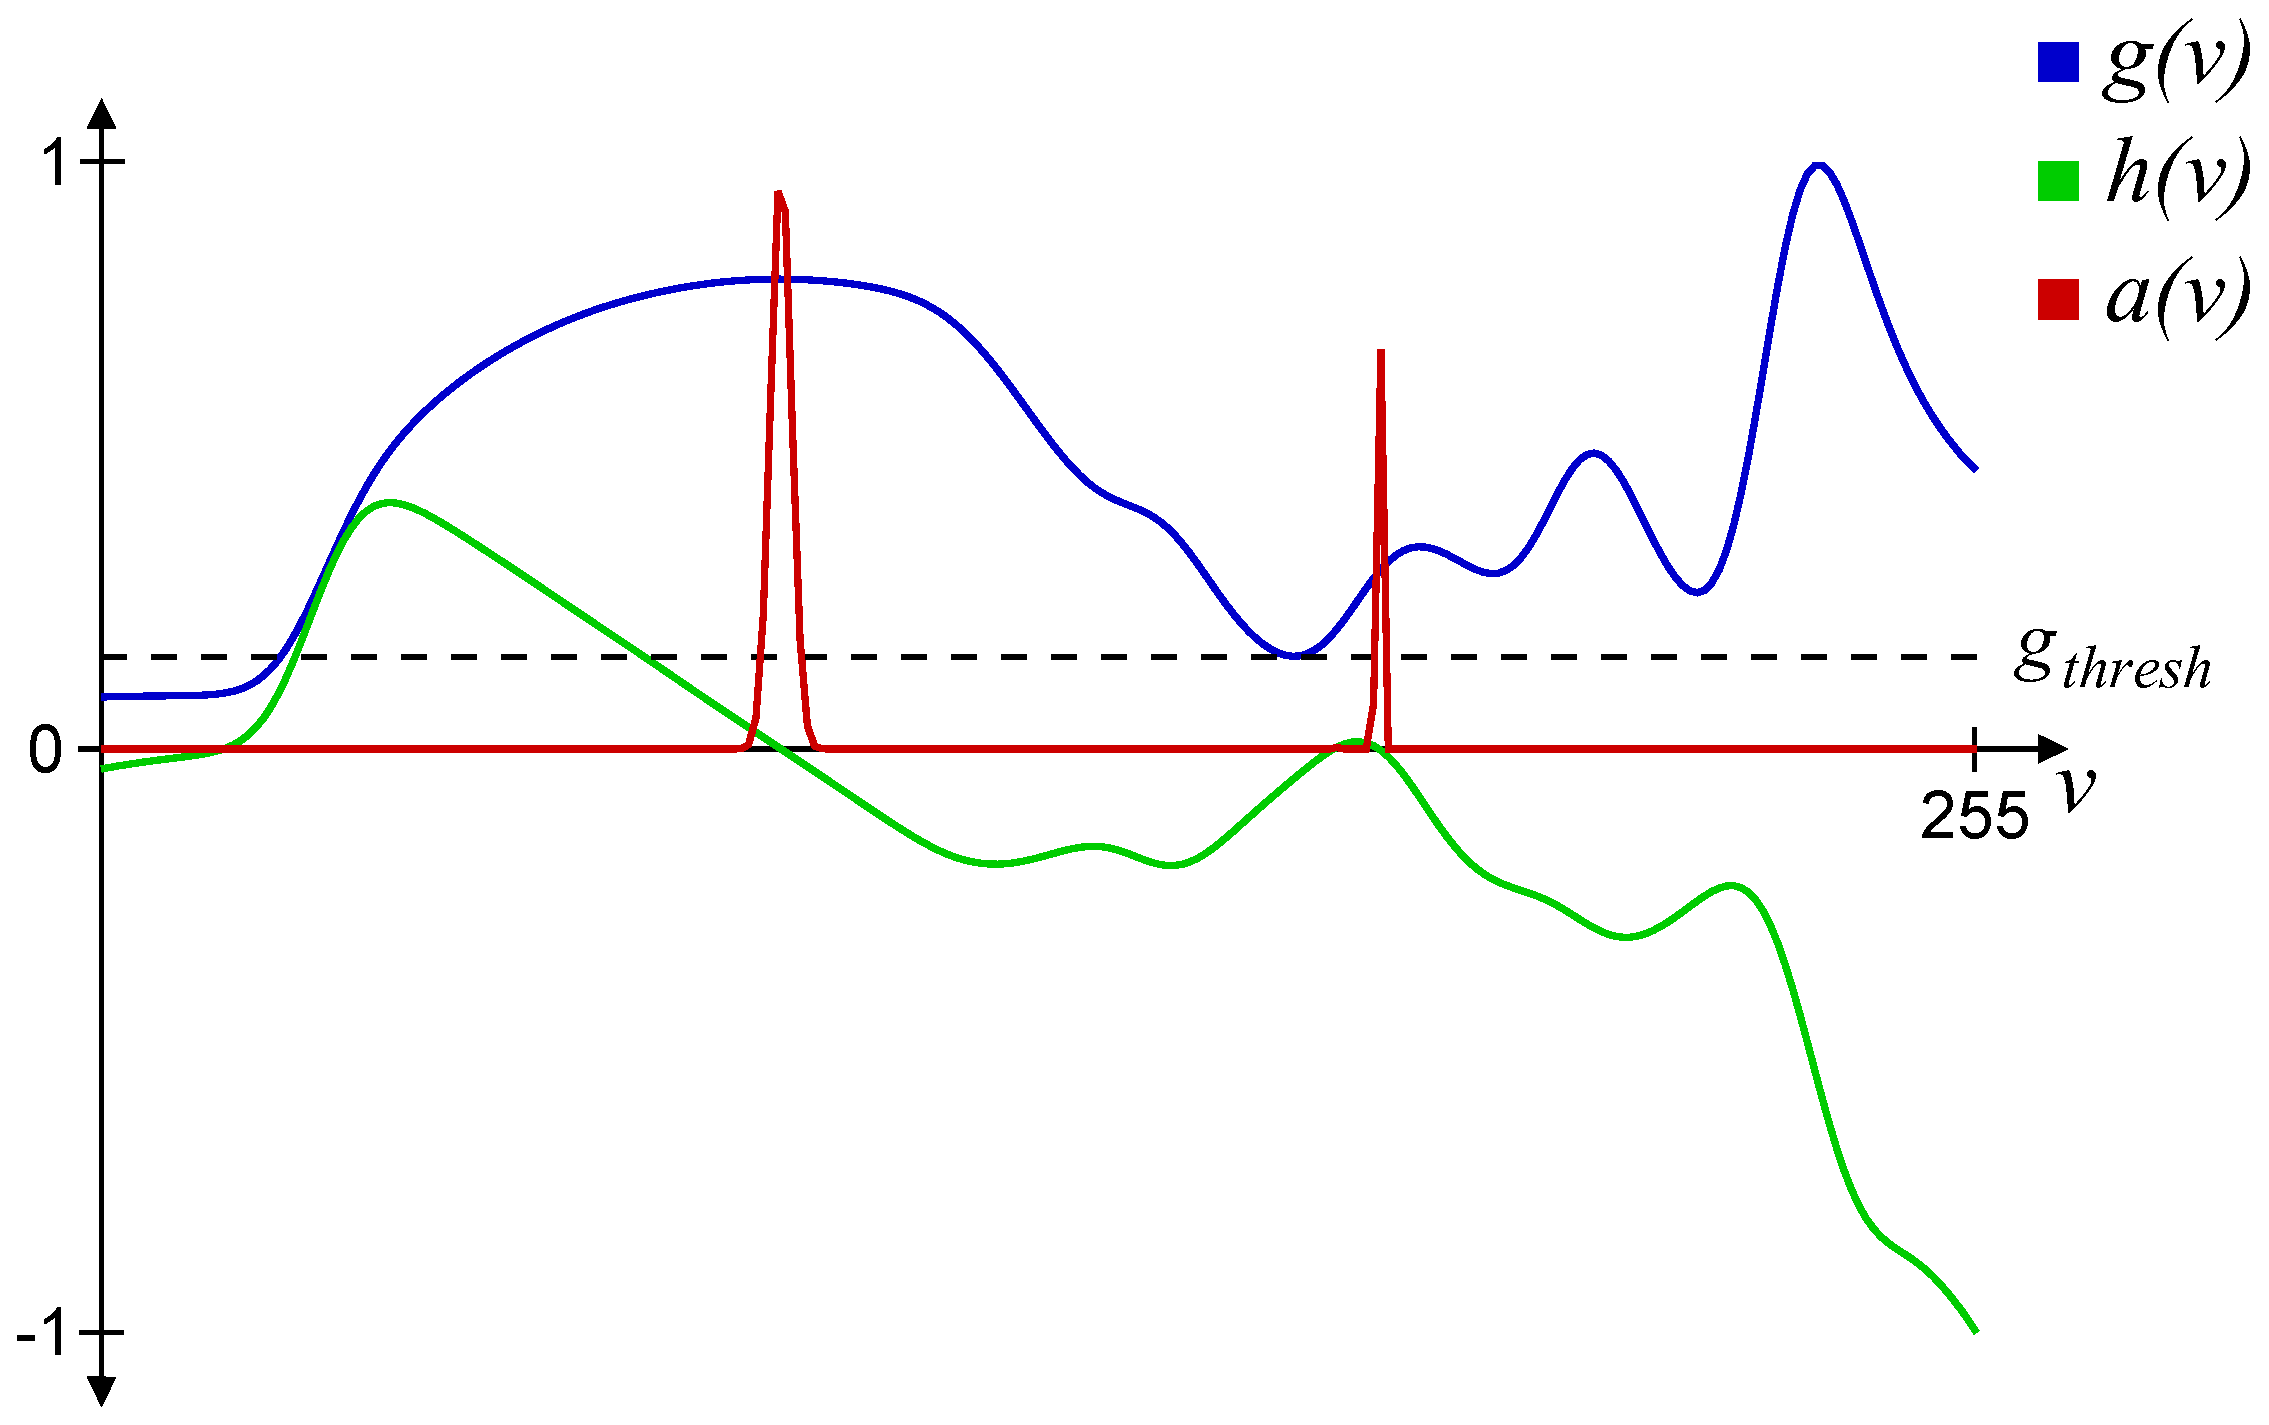
\includegraphics[width=0.65\textwidth]{images/r_g_3sphere_ft}
		\label{fig:r_3sphere_kd}
	}
	\subfigure[Método proposto.]
	{
		\includegraphics[width=0.35\textwidth]{images/r_m_3sphere}
		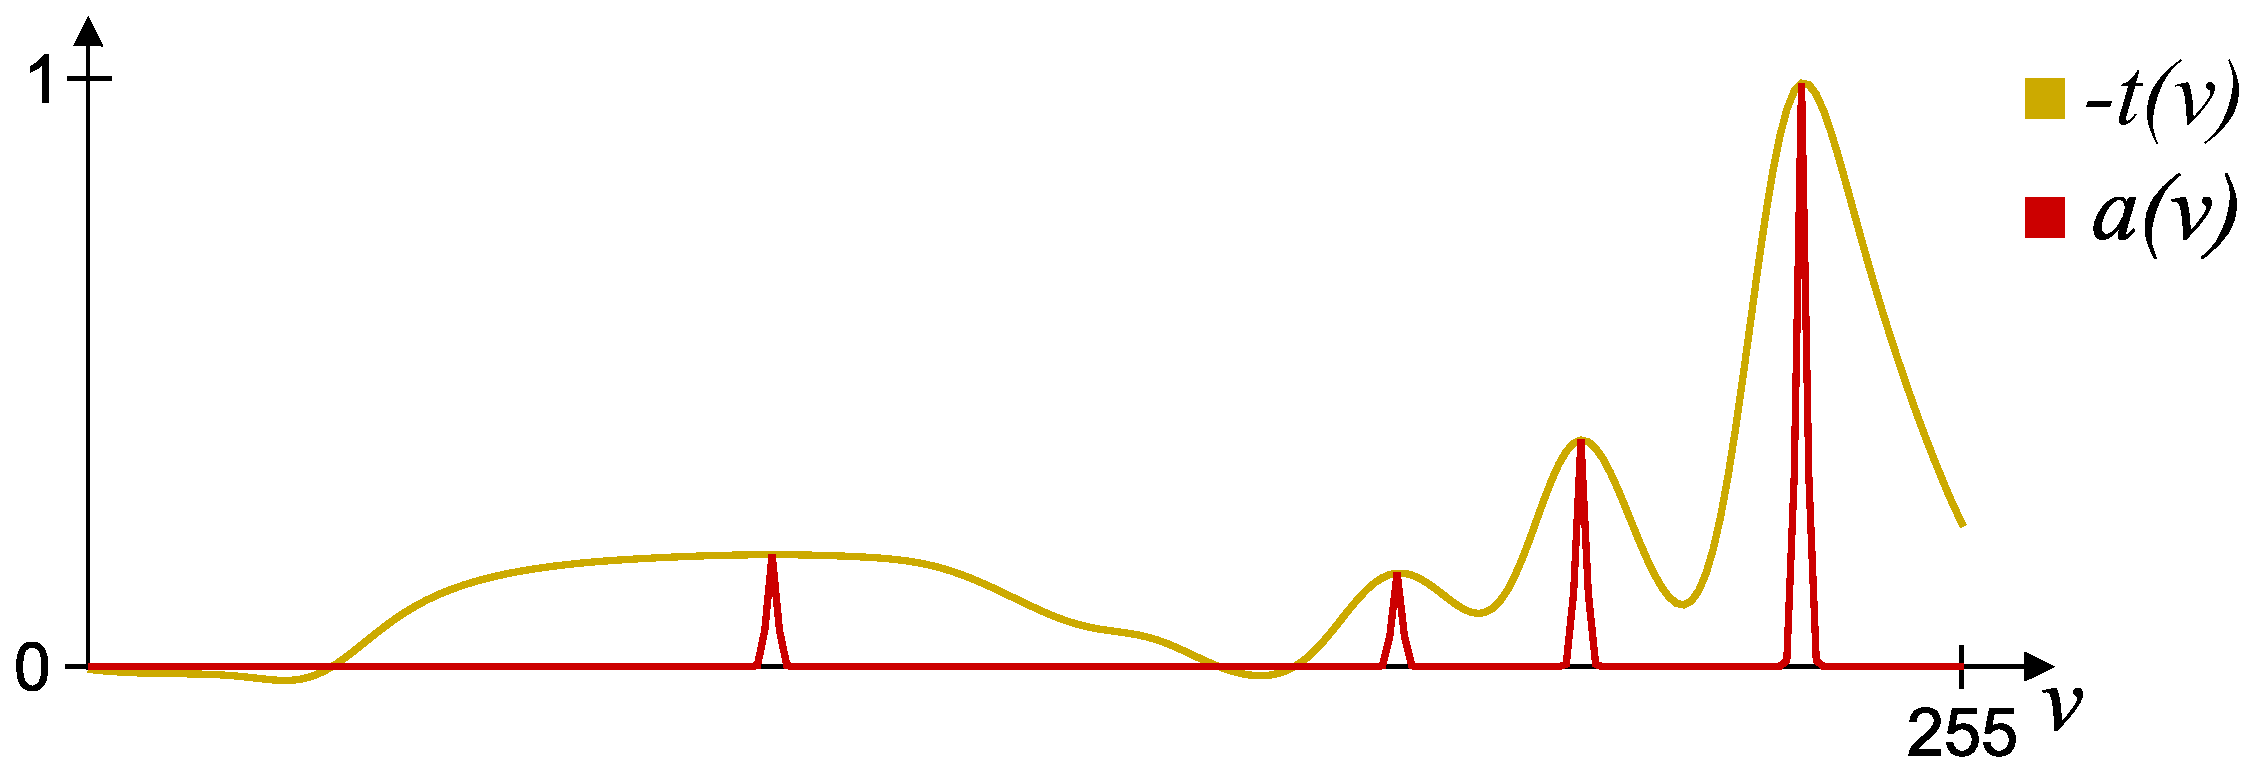
\includegraphics[width=0.65\textwidth]{images/r_m_3sphere_ft}			\label{fig:r_3sphere_mine}
	}
	\caption{Visualização e função de transferência do volume \quote{Test Spheres}.}
	\label{fig:r_3sphere}
\end{figure}

%%%%%%%%%%%%%%%%%%%%%%%%%%%%%%%%%% NUCLEON %%%%%%%%%%%%%%%%%%%%%%%%%%%%%%%%%%%%%
	A Figura~\ref{fig:r_nucleon_slice} mostra uma fatia do volume \quote{Nucleon}. Nela é possível observar duas fronteiras: preto-cinza, cinza-branco. A Figura~\ref{fig:r_nucleon}~\ref{fig:r_nucleon_kd} mostra que o método de \textit{Kindlmann e Durkin} identifica apenas uma fronteira, enquanto o método proposto por esta dissertação identifica as duas existentes, como mostra a Figura~\ref{fig:r_nucleon}~\ref{fig:r_nucleon_mine}. Contudo, ao comparar a fatia do volume com as visualizações, observa-se que a isosuperfície esférica central é mais fielmente representada pela fronteira destacada pelo método de \textit{Kindlmann e Durkin}.
	
\begin{figure}[h]
	\centering
	\includegraphics[width=0.33\textwidth]{images/g_nucleon_slice}
	\caption{Fatia do volume \quote{Nucleon}.}
	\label{fig:r_nucleon_slice}
\end{figure}

\begin{figure}[h]
	\centering
	\subfigure[Método de \textit{Kindlmann e Durkin}.]
	{
		\includegraphics[width=0.3\textwidth]{images/g_nucleon}
		\includegraphics[width=0.65\textwidth]{images/r_g_nucleon_ft}
		\label{fig:r_nucleon_kd}
	}
	\subfigure[Método proposto.]
	{
		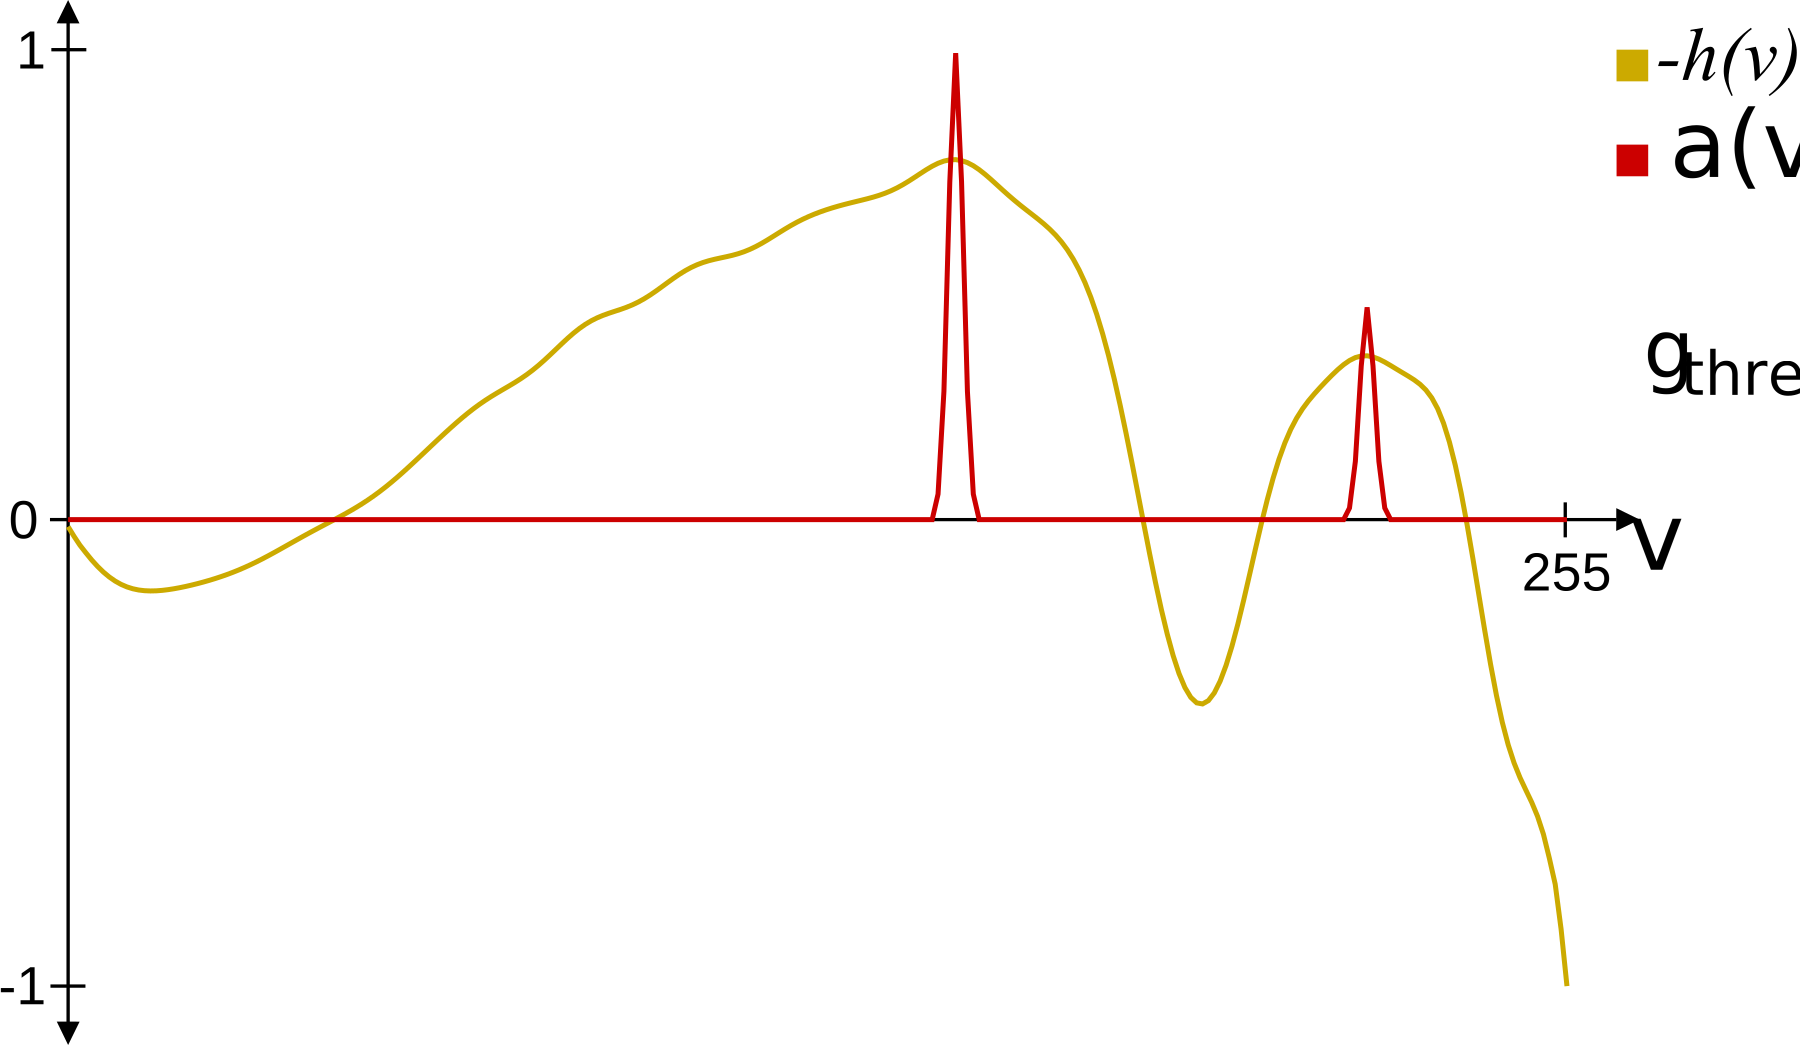
\includegraphics[width=0.3\textwidth]{images/r_m_nucleon}
		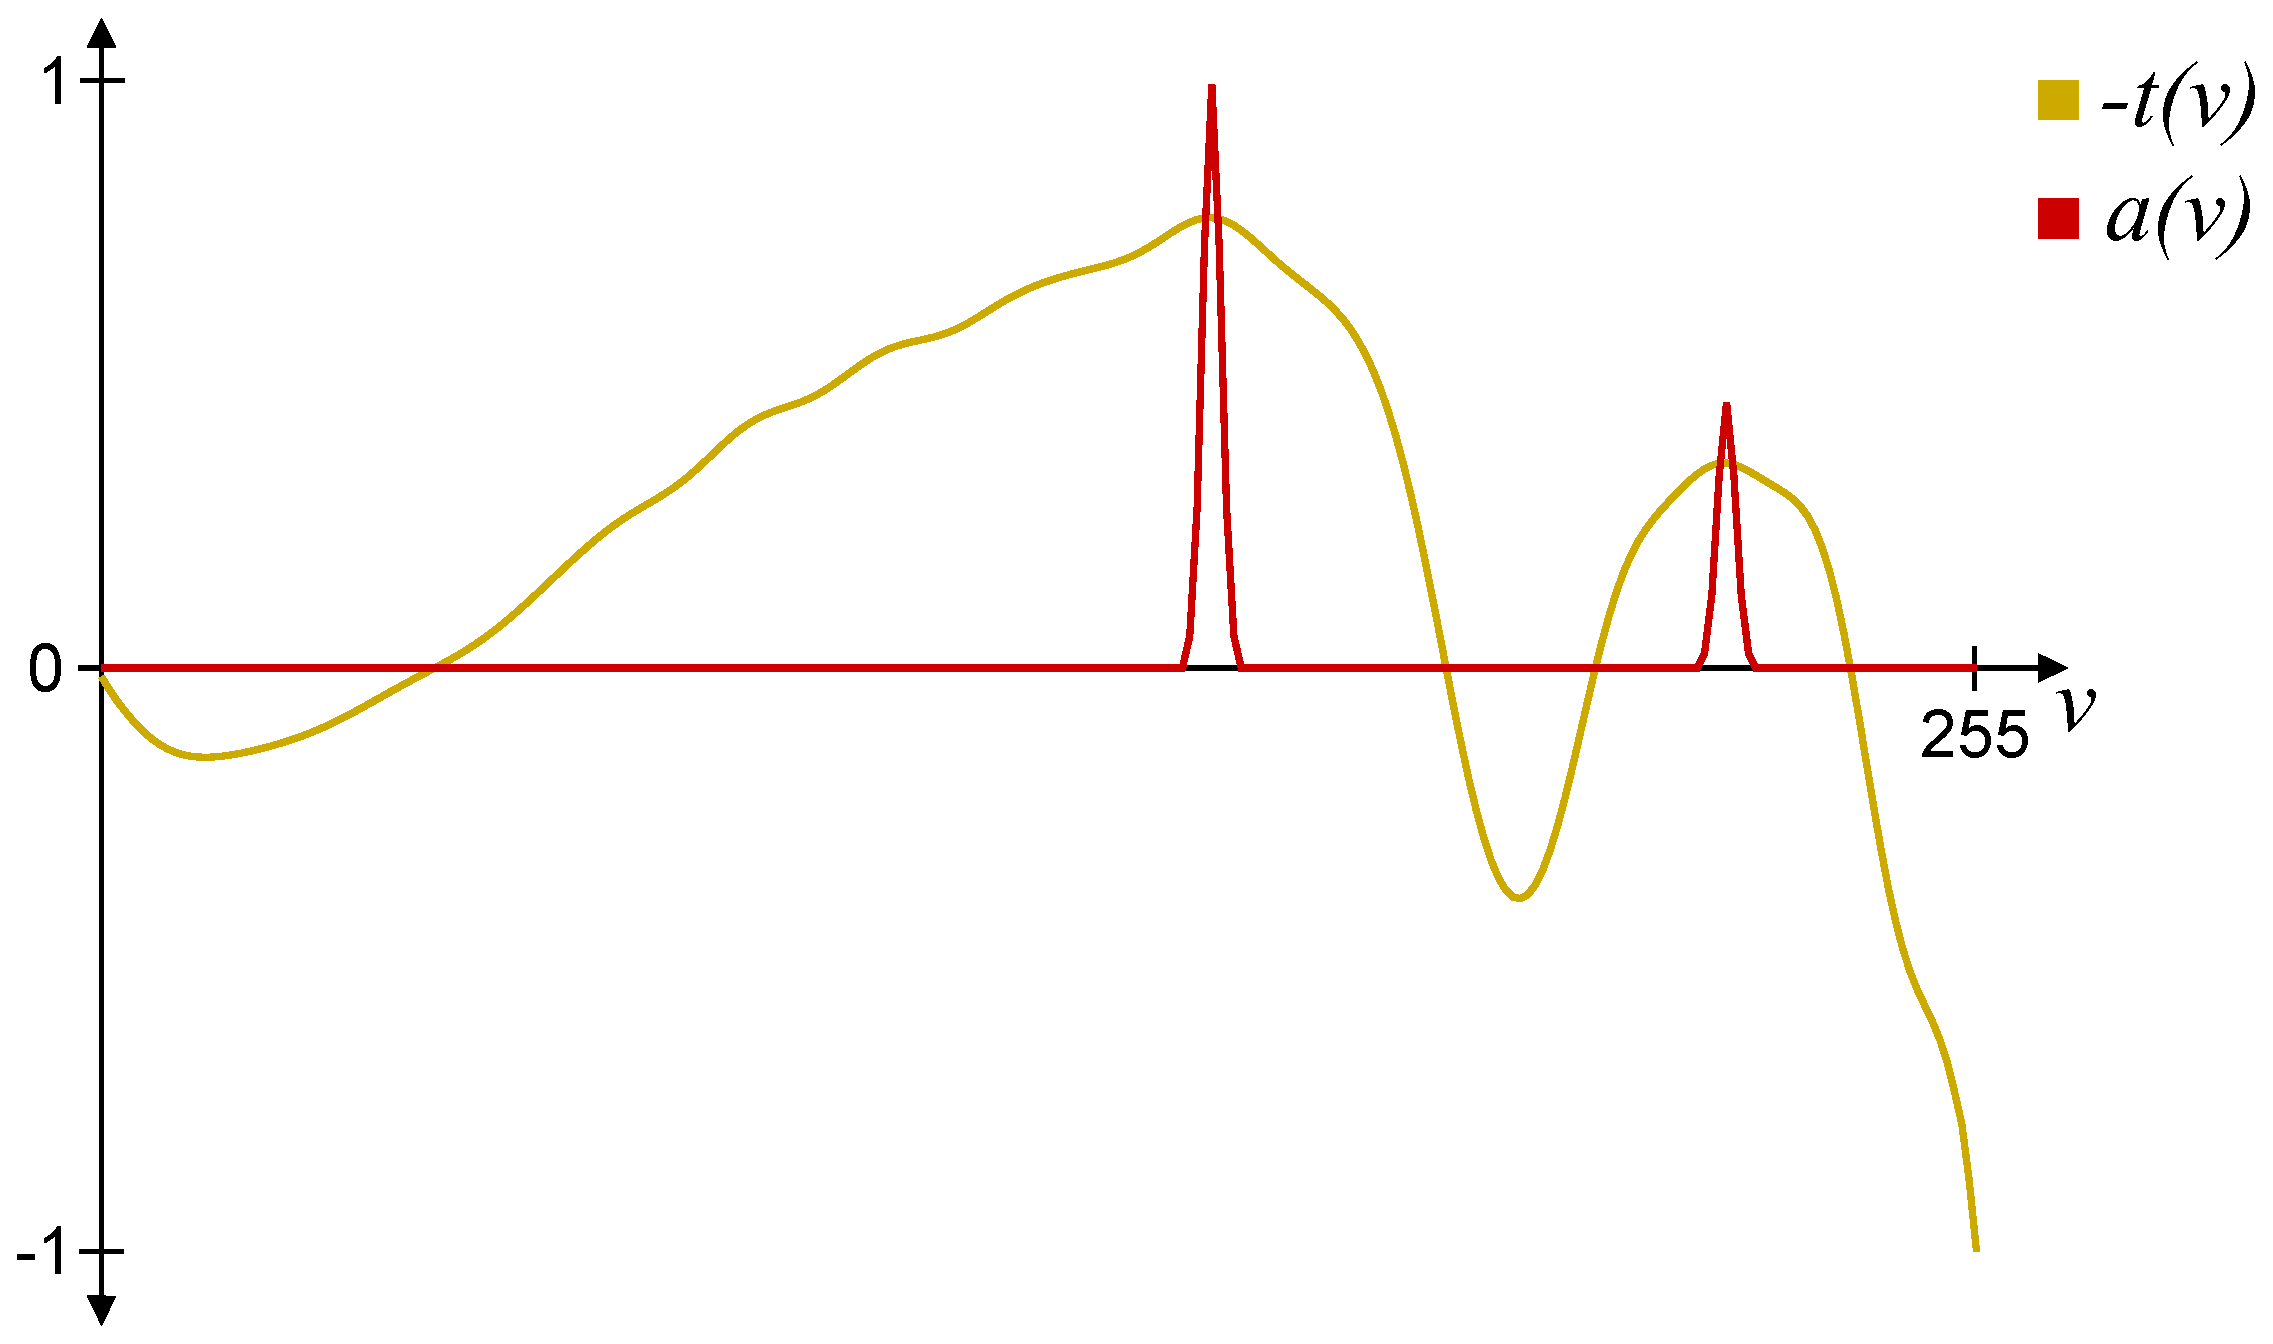
\includegraphics[width=0.65\textwidth]{images/r_m_nucleon_ft}			\label{fig:r_nucleon_mine}
	}
	\caption{Visualização e função de transferência do volume \quote{Nucleon}.}
	\label{fig:r_nucleon}
\end{figure}
	
%%%%%%%%%%%%%%%%%%%%%%%%%%%%%%%%%% ENGINE %%%%%%%%%%%%%%%%%%%%%%%%%%%%%%%%%%%%%
%	A Figura~\ref{fig:r_engine_slice} exibe uma fatia do volume \quote{Engine}, onde pode ser observada a existência de $ 3 $ fronteiras. Comparando as visualizações resultantes dos dois métodos, exibidas na Figura~\ref{fig:r_engine}, percebe-se que ambos foram capazes de realçar corretamente as fronteiras do volume. No entanto, ressalta-se que esta equivalência só foi possível após encontrar o valor de $ g_{thresh} $ que eliminou algumas regiões da visualização do método de \textit{Kindlmann e Durkin} que foram realçadas indevidamente, devido ao deslocamento do segundo pico da sua função de transferência.
%
%\begin{figure}[h]
%	\centering
%	\subfigure[Método de \textit{Kindlmann e Durkin}.]
%	{
%		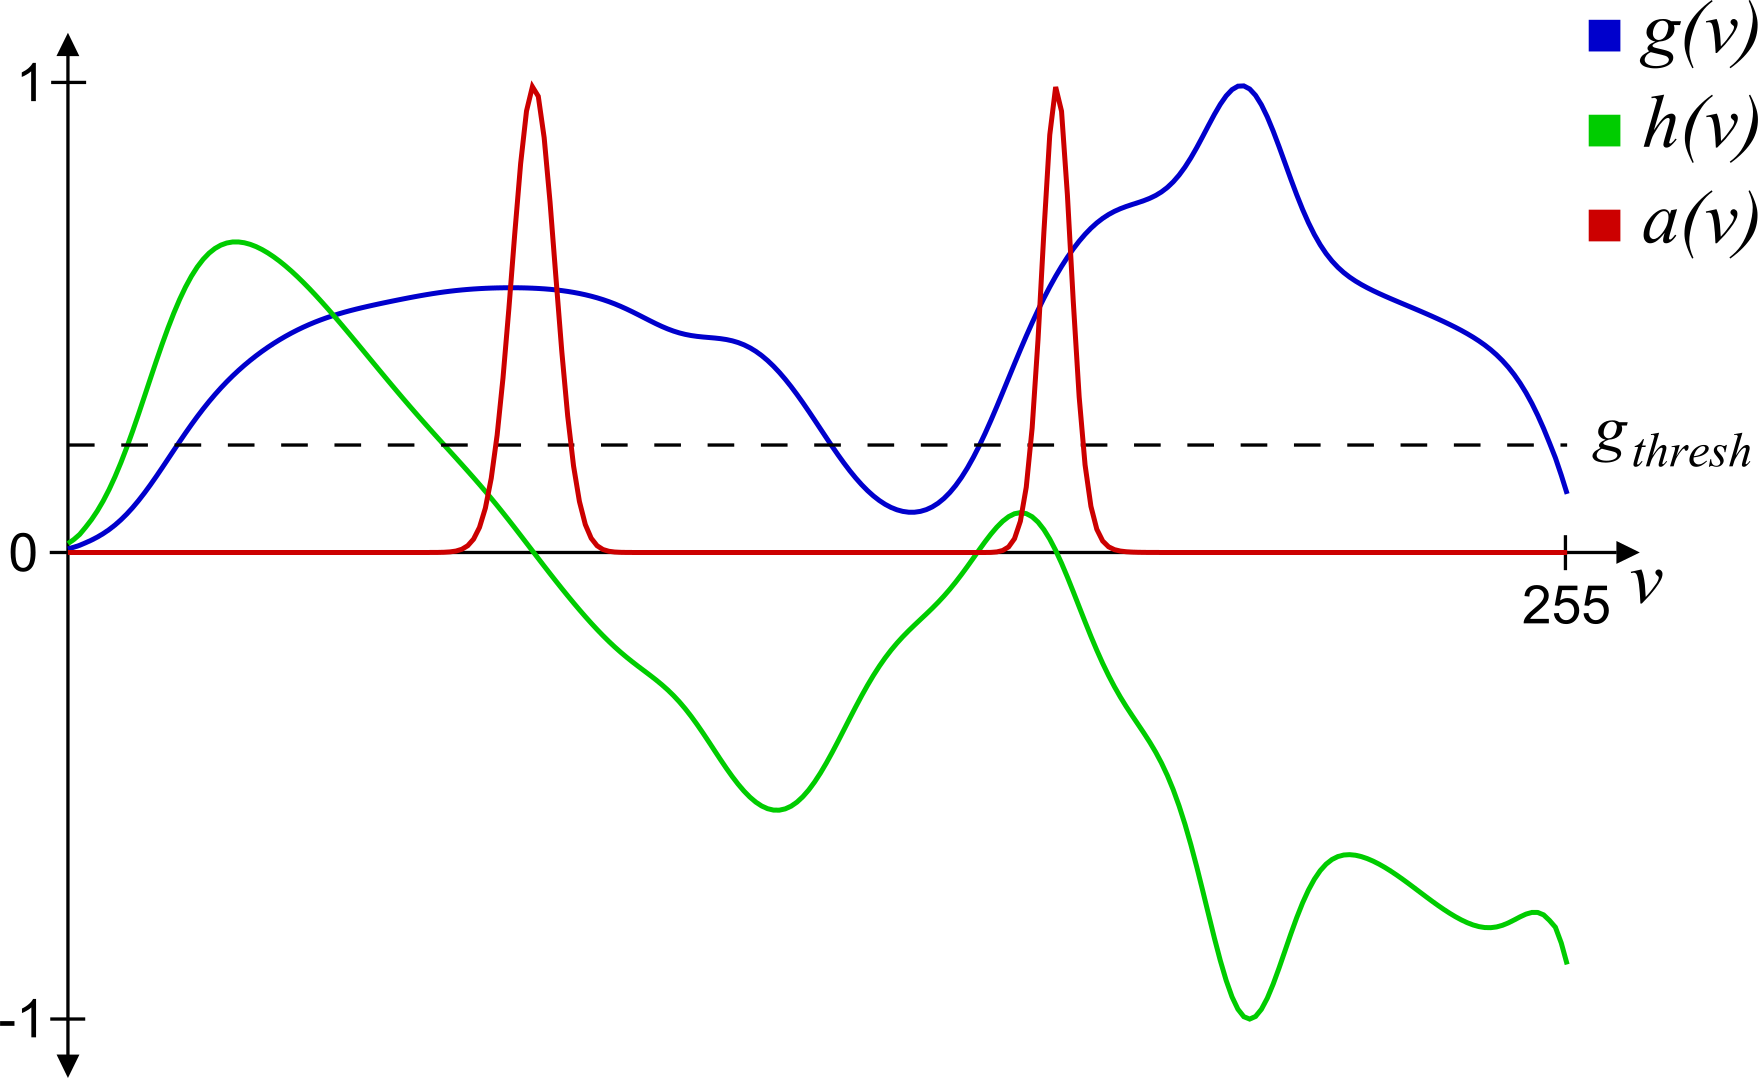
\includegraphics[width=0.35\textwidth]{images/r_g_engine}
%		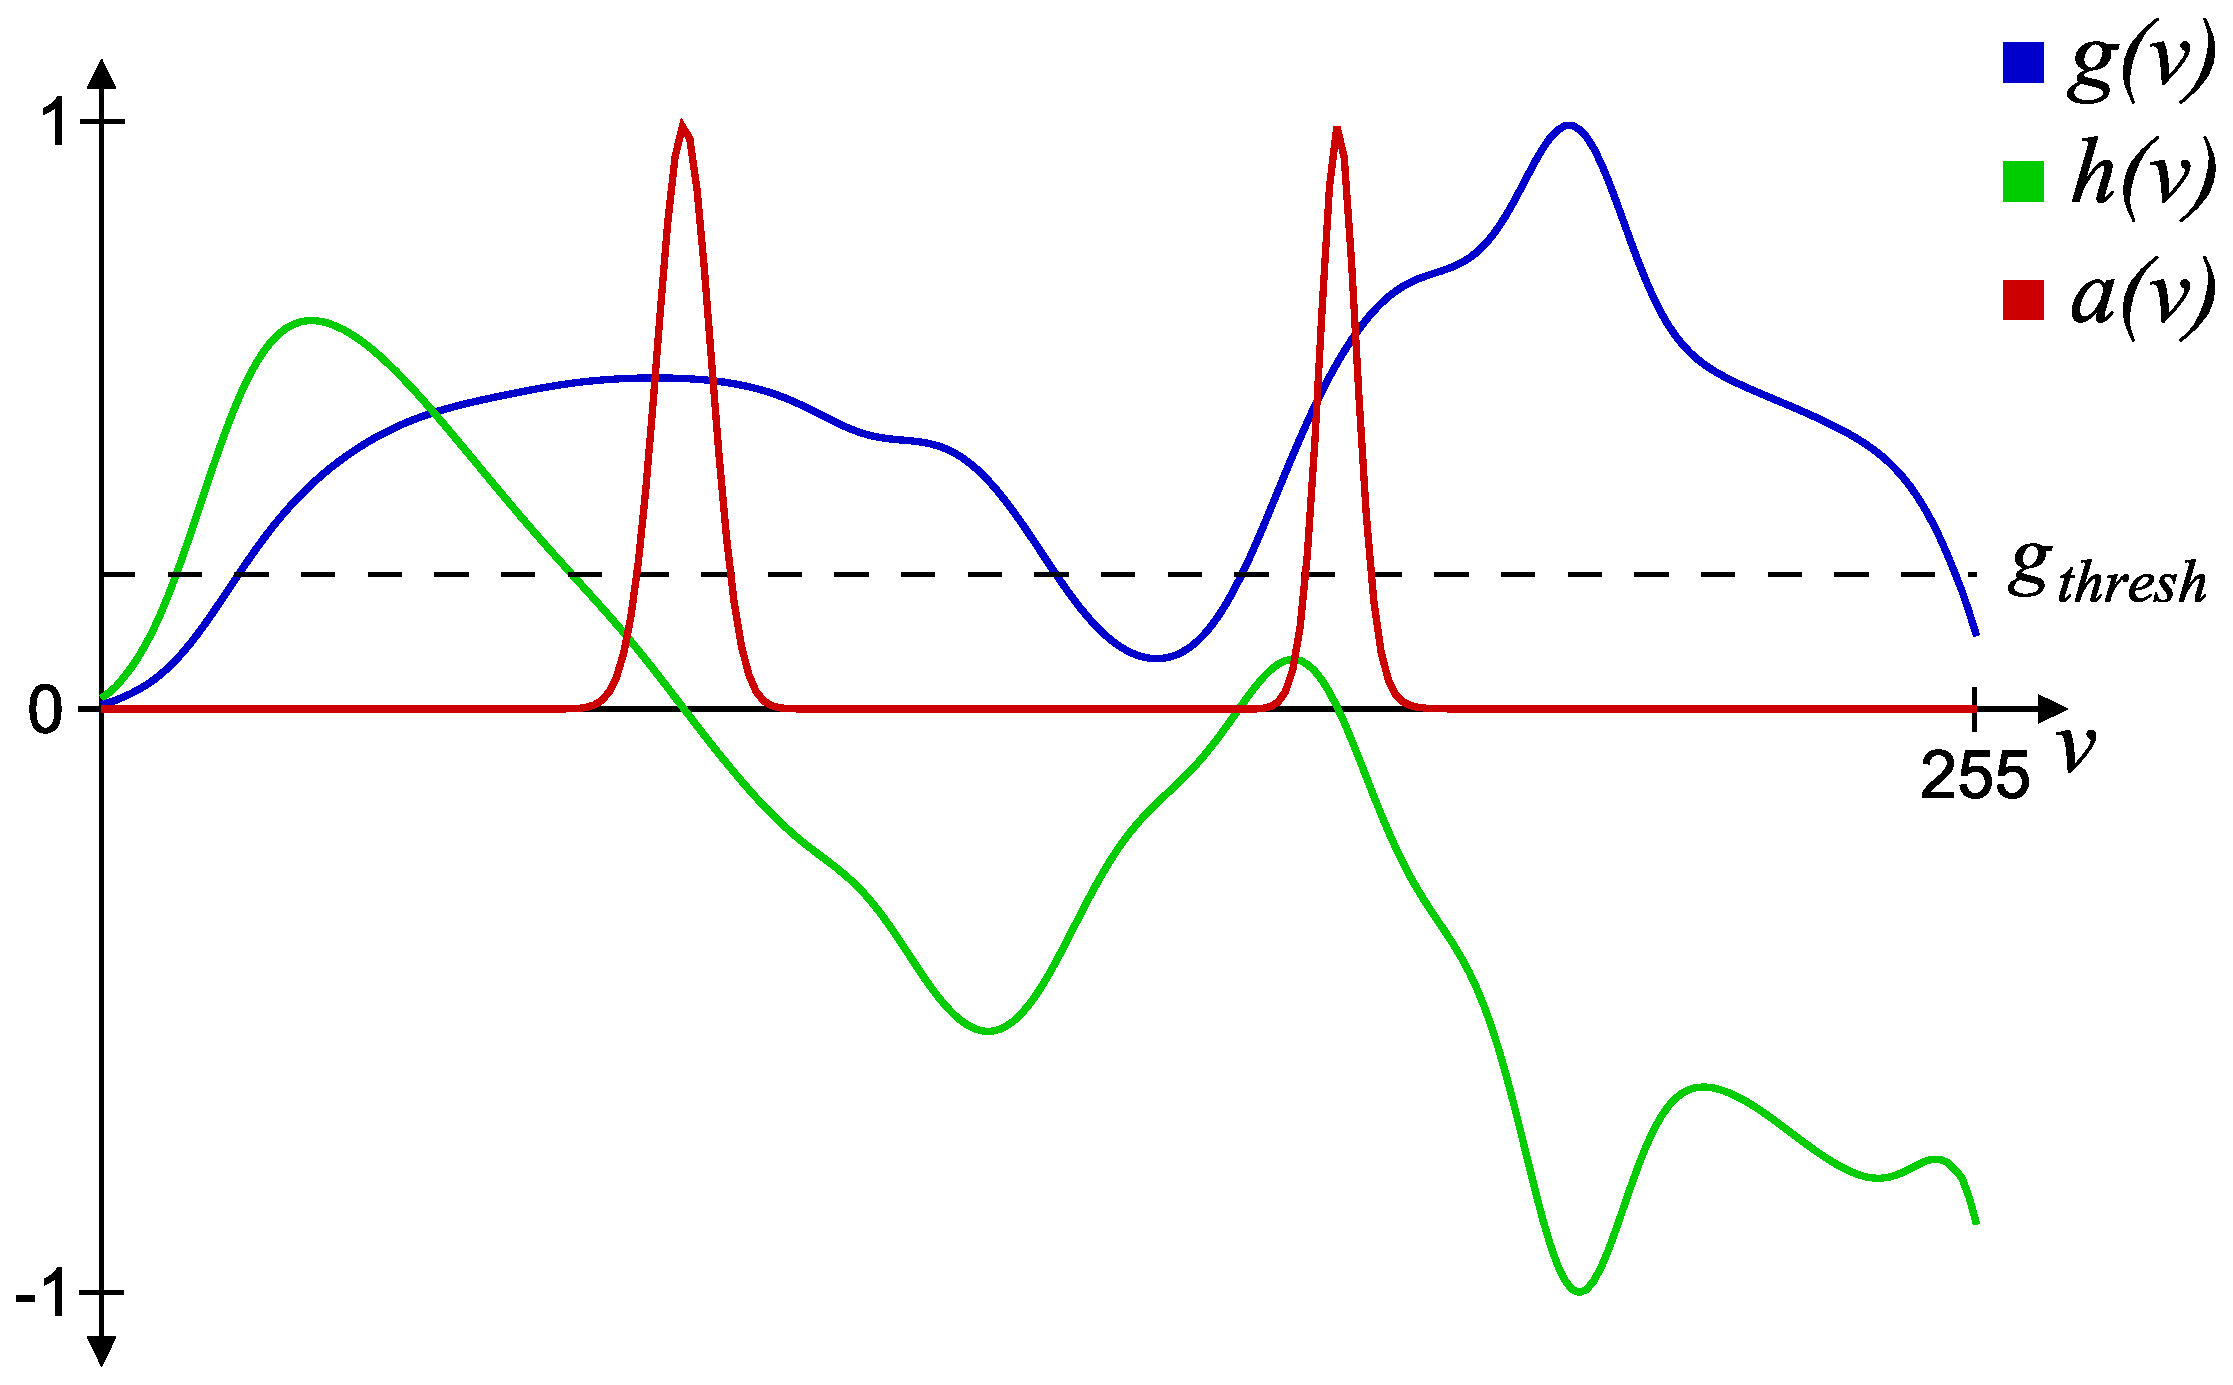
\includegraphics[width=0.65\textwidth]{images/r_g_engine_ft}
%		\label{fig:r_engine_kd}
%	}
%	\subfigure[Método proposto.]
%	{
%		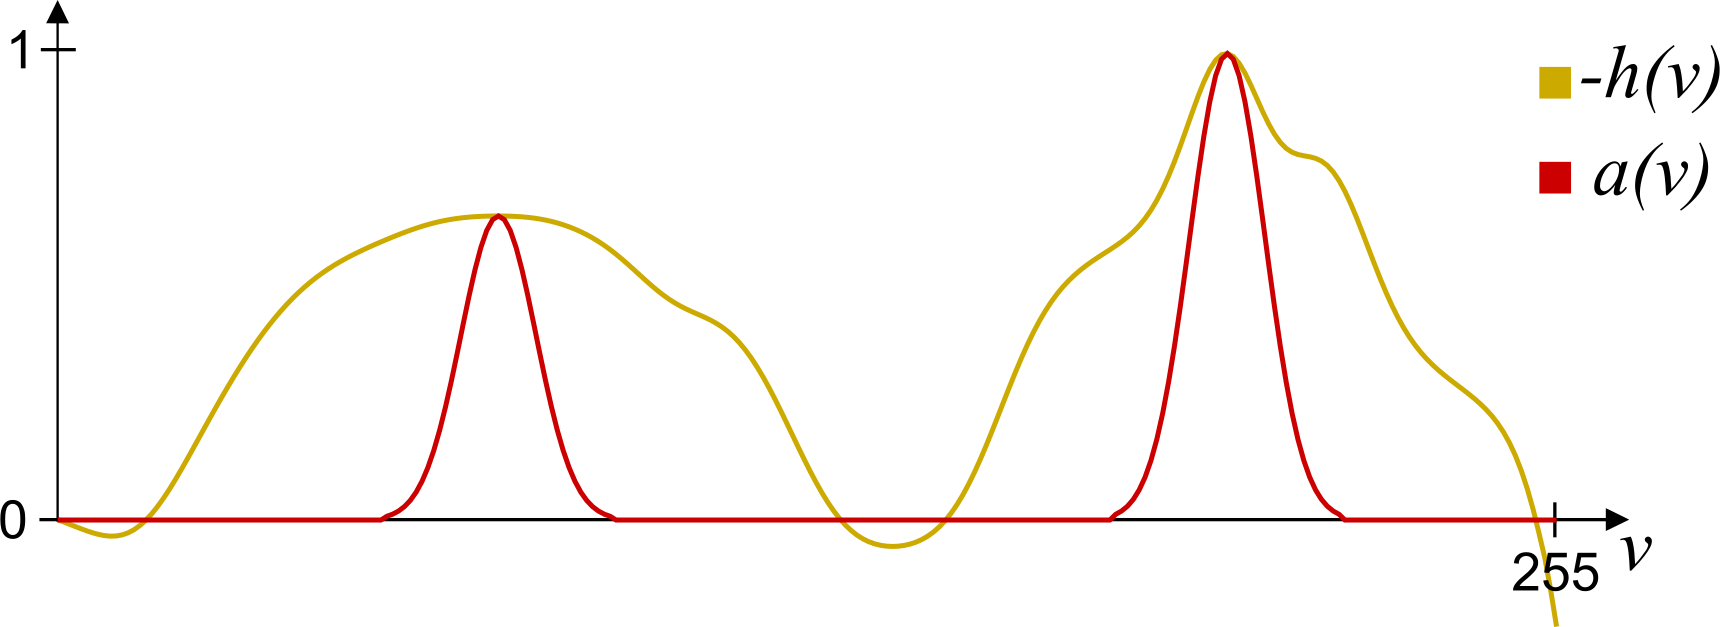
\includegraphics[width=0.35\textwidth]{images/r_m_engine}
%		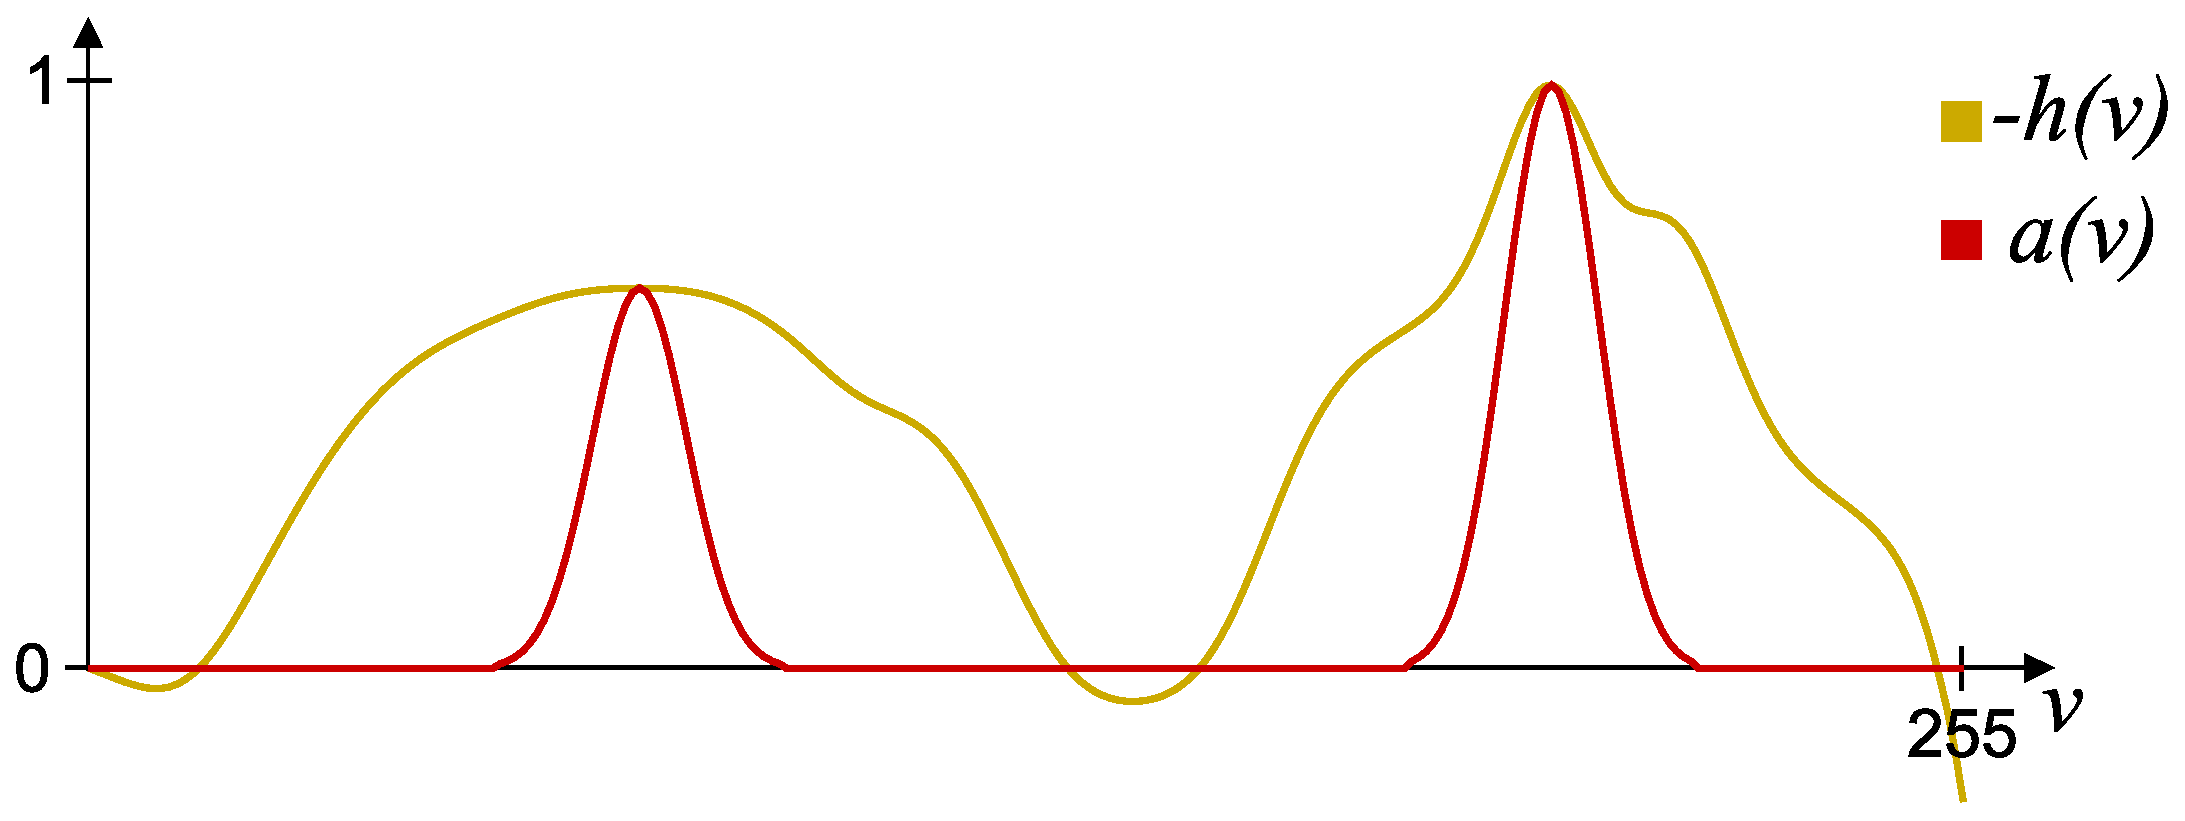
\includegraphics[width=0.65\textwidth]{images/r_m_engine_ft}			\label{fig:r_engine_mine}
%	}
%	\caption{Visualização e função de transferência do volume \quote{Engine}.}
%	\label{fig:r_engine}
%\end{figure}
%%%%%%%%%%%%%%%%%%%%%%%%%%%%%%%%%% CT HEAD %%%%%%%%%%%%%%%%%%%%%%%%%%%%%%%%%%%%%
	O volume a seguir é uma tomografia computadorizada de uma cabeça com uma estrutura de suporte na parte de trás. A Figura~\ref{fig:r_cthead} mostra que os dois métodos realçam a cabeça, o crânio e a estrutura de suporte. O segundo pico das duas funções de transferência são coincidentes e equivalem ao crânio, em amarelo. No entanto, o primeiro pico não coincide.
	
	O método de \textit{Kindlmann~e~Durkin} apresenta um deslocamento para a esquerda, centralizando esse pico onde a segunda derivada é igual a zero. Devido à posição desse pico (que não ocorre junto a um máximo local na primeira derivada média), alguns voxels do volume são realçados juntamente com a cabeça e sua estrutura de suporte, permitindo a interpretação de que todos compõem uma só isosuperfície. O mesmo não ocorre com o método proposto por esta dissertação, que realça a cabeça corretamente ao mesmo tempo que mostra menos a estrutura presente na sua parte de trás, permitindo entendê-las como isosuperfícies diferentes.

\begin{figure}[h]
	\centering
	\subfigure[Método de \textit{Kindlmann e Durkin}.]
	{
		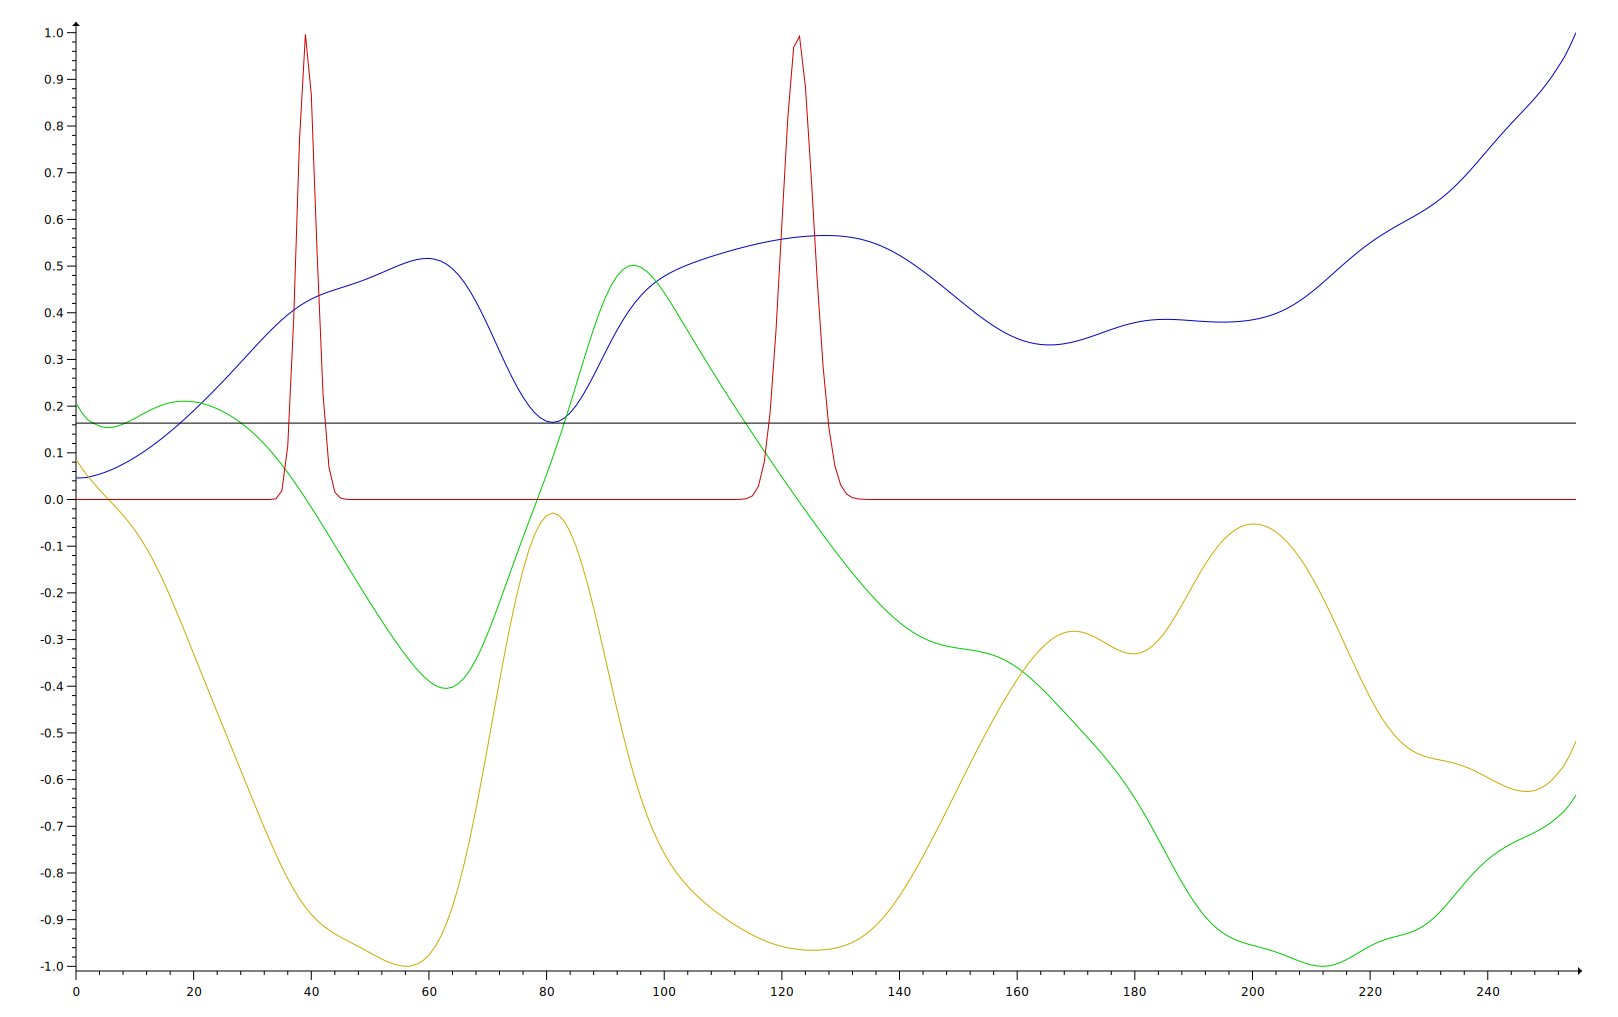
\includegraphics[width=0.35\textwidth]{images/r_g_cthead}
		\includegraphics[width=0.65\textwidth]{images/r_g_cthead_ft}
		\label{fig:r_cthead_kd}
	}
	\subfigure[Método proposto.]
	{
		\includegraphics[width=0.35\textwidth]{images/r_m_cthead}
		\includegraphics[width=0.65\textwidth]{images/r_m_cthead_ft}			\label{fig:r_cthead_mine}
	}
	\caption{Visualização e função de transferência do volume \quote{CT Head}.}
	\label{fig:r_cthead}
\end{figure}

	O terceiro pico da função de transferência na Figura~\ref{fig:r_cthead}~\ref{fig:r_cthead_mine} destaca incorretamente uma isosuperfície, pois ela não corresponde a uma fronteira. Ao isolá-la, vê-se uma estrutura semelhante ao crânio, porém incompleta. Já a quarta fronteira foi obtida corretamente e realça os dentes. A Figura~\ref{fig:r_cthead_iso} mostra a visualização apenas do crânio, que pode ser obtida através da interface, selecionando apenas a segunda fronteira.

\begin{figure}[h]
	\centering
	\subfigure[Função de transferência.]
	{
		\includegraphics[width=0.8\textwidth]{images/r_m_cthead_iso_ft}
	}
	\subfigure[Visualização volumétrica.]
	{
		\includegraphics[width=0.7\textwidth]{images/r_m_cthead_iso}
	}
	\caption{Realce do crânio do volume \quote{CT Head} através da interface.}
	\label{fig:r_cthead_iso}
\end{figure}

%%%%%%%%%%%%%%%%%%%%%%%%%%%%%%%%%% Tooth %%%%%%%%%%%%%%%%%%%%%%%%%%%%%%%%%%%%%

	O volume seguinte é um dente envolvido por um material que causa a forma cilíndrica revelada nas visualizações da Figura~\ref{fig:r_tooth}. Como pode ser observado, tanto as funções de transferência como suas respectivas visualizações são semelhantes em ambos os métodos. Percebe-se apenas um ligeiro deslocamento da última fronteira obtida pelo método de \textit{Kindlmann~e~Durkin}, resultando em uma isosuperfície laranja mais forte que a encontrada pelo método aqui proposto.
	
\begin{figure}[h]
	\centering
	\subfigure[Método de \textit{Kindlmann e Durkin}.]
	{
		\includegraphics[width=0.35\textwidth]{images/r_g_tooth}
		\includegraphics[width=0.65\textwidth]{images/r_g_tooth_ft}
		\label{fig:r_tooth_kd}
	}
	\subfigure[Método proposto.]
	{
		\includegraphics[width=0.35\textwidth]{images/r_m_tooth}
		\includegraphics[width=0.65\textwidth]{images/r_m_tooth_ft}			\label{fig:r_tooth_mine}
	}
	\caption{Visualização e função de transferência de um dente.}
	\label{fig:r_tooth}
\end{figure}

%%%%%%%%%%%%%%%%%%%%%%%%%%%%%%%%%% Bonsai %%%%%%%%%%%%%%%%%%%%%%%%%%%%%%%%%%%%%
	O bonsai já é um volume conhecido na literatura, principalmente pelo ruído presente acima das raízes, que possui valor muito próximo ao das folhas. Portanto, para visualizá-lo corretamente, é preciso remover as isosuperfícies que correspondem a esse ruído e aumentar a largura da função de transferência até que até que as folhas apareçam novamente. No método 1D de \textit{Kindlmann~e~Durkin} esse processo é feito através do $ g_{thresh} $, enquanto no método desta dissertação desliga-se as isosuperfícies através da interface, como já explicado na Seção~\ref{sec:my.tf}.
	
	Como pode ser observado na Figura~\ref{fig:r_m_bonsai}, as funções de transferência são bem distintas, apesar de resultarem em visualizações quase idênticas. Então, cabe observar que, dentro da proposta de realçar como fronteira a isosuperfície que possui maior derivada, o método proposto por esta dissertação apresenta uma função de transferência mais adequada.
	
\begin{figure}[h]
	\centering
	\subfigure[Método de \textit{Kindlmann e Durkin}.]
	{
		\includegraphics[width=0.7\textwidth]{images/r_g_bonsai_ft}
		\label{fig:r_bonsai_kd_ft}
	}
	\subfigure[Método proposto.]
	{
		\includegraphics[width=0.7\textwidth]{images/r_m_bonsai_ft}			\label{fig:r_bonsai_mine_ft}
	}
	\subfigure[Método de \textit{Kindlmann e Durkin}.]
	{
		\includegraphics[width=0.47\textwidth]{images/r_g_bonsai}
		\label{fig:r_bonsai_kd}
	}
	\subfigure[Método proposto.]
	{
		\includegraphics[width=0.47\textwidth]{images/r_m_bonsai}
		\label{fig:r_bonsai_mine}
	}
	\caption{Visualização e função de transferência do bonsai.}
	\label{fig:r_m_bonsai}
\end{figure}

%%%%%%%%%%%%%%%%%%%%%%%%%%%%%%%%%% X %%%%%%%%%%%%%%%%%%%%%%%%%%%%%%%%%%%%%
\clearpage
	Os dois volumes seguintes apresentam a mesma situação ocorrida com o bonsai no momento de comparar os dois métodos: funções de transferência diferentes que resultam em visualizações muito parecidas. Por isso, serão apresentados apenas os resultados oriundos do método proposto nesta dissertação.
	
	A Figura~\ref{fig:r_m_carp} mostra a função de transferência obtida com o método desta dissertação, bem como a visualização volumétrica resultante. As duas primeiras fronteiras vistas na FT correspondem respectivamente ao exterior e ao exoesqueleto da carpa. As outras duas representam regiões pequenas do exoesqueleto de maior intensidade. A Figura~\ref{fig:r_m_carp}~\ref{fig:r_m_carp_exo} mostra apenas o exoesqueleto da carpa. Para isso, a fronteira referente ao exterior da carpa foi desligada e a opacidade máxima da função de transferência aumentada.
	
\begin{figure}[h]
	\centering
	\subfigure[]
	{
		\includegraphics[width=0.7\textwidth]{images/r_m_carp_ft}
		\label{fig:r_m_carp_ft}
	}
	\subfigure[]
	{
		\includegraphics[width=0.8\textwidth]{images/r_m_carp}
		\label{fig:r_m_carp_side}
	}
	\subfigure[]
	{
		\includegraphics[width=0.8\textwidth]{images/r_m_carp_up}
		\label{fig:r_m_carp_up}
	}
	\subfigure[]
	{
		\includegraphics[width=0.8\textwidth]{images/r_m_carp_exo}
		\label{fig:r_m_carp_exo}
	}
	\caption{Carpa.}
	\label{fig:r_m_carp}
\end{figure}

%\begin{figure}[h]
%	\centering
%	\subfigure[]
%	{
%		\includegraphics[width=0.7\textwidth]{images/r_m_carp_exo_ft}
%	}
%	\subfigure[]
%	{
%		\includegraphics[width=0.8\textwidth]{images/r_m_carp_exo}
%	}	
%	\caption{Exoesqueleto da carpa.}
%	\label{fig:r_m_carp_exo}
%\end{figure}

	No volume \quote{Knee}, assim como no bonsai, foi preciso manipular a função de transferência em ambos os métodos para se obter apenas o osso. Então, desligou-se o pico da função de transferência que não correspondia aos ossos dos joelhos. Como neste volume, a intensidade da estrutura óssea abrange um grande intervalo de valores, foi preciso aumentar consideravelmente a largura da gaussiana.

\begin{figure}[h]
	\centering
	\subfigure[]
	{
		\includegraphics[width=0.7\textwidth]{images/r_m_knee_ft}
	}
	\subfigure[]
	{
		\includegraphics[width=0.8\textwidth]{images/r_m_knee}
	}
	\caption{Volume médico de joelhos.}
\end{figure}

\clearpage
\section{Malhas Não Regulares}
\label{sec:result.irreg}

	Nesta seção, são exibidos os resultados para dois modelos simples (A e B) de reservatório e um modelo real (Pituba). Para visualizar esses volumes com malhas não regulares, escolheu-se a técnica proposta por \textit{Miranda e Celes}~\cite{miranda}.
	
%%%%%%%%%%%%%%%%%%%%%%%%%%%%%%%%% VREP SO 1 %%%%%%%%%%%%%%%%%%%%%%%%%%%%%%%%%%%%
	A Figura~\ref{fig:box_slice} mostra a simulação da saturação de óleo (SO) para o modelo de reservatório A. As fronteiras fortes podem ser identificadas por regiões próximas de coloração diferente, onde suas respectivas cores não são vizinhas na escala de cores. Quanto maior a distância na escala de cores, mais forte é a fronteira. Portanto, percebe-se que este modelo possui uma fronteira forte entre o amarelo e o vermelho.\\
	
\begin{figure}[h]
	\centering
	\includegraphics[width=1\textwidth]{images/r_vrep_so_slice}
	\caption{Fatia do volume de SO do modelo A.}
	\label{fig:box_slice}
\end{figure}

	A Figura~\ref{fig:r_vrep} mostra que os dois métodos identificam a fronteira mais forte. Além disso, ambos destacam também uma fronteira em azul, próximo ao posso injetor. Contudo, o método descrito por esta dissertação identifica também uma terceira fronteira, que representa a fronteira entre a região vermelha e a laranja, na Figura~\ref{fig:box_slice}. Por conta desta última fronteira, uma outra isosuperfície (em vermelho) é realçada próxima à fronteira mais forte. O mesmo ocorre com o método de \textit{Kindlmann e Durkin}, que realça uma isosuperfície pequena (semelhante a um traço) no canto inferior direito da visualização da Figura~\ref{fig:r_vrep}~\ref{fig:r_vrep_kd}

\begin{figure}[h]
	\centering
	\subfigure[Método de \textit{Kindlmann e Durkin}.]
	{
		\includegraphics[width=0.35\textwidth]{images/r_vrep_so_kd}
		\includegraphics[width=0.65\textwidth]{images/r_vrep_so_kd_ft}
		\label{fig:r_vrep_kd}
	}
	\subfigure[Método proposto.]
	{
		\includegraphics[width=0.35\textwidth]{images/r_vrep_so_mine}
		\includegraphics[width=0.65\textwidth]{images/r_vrep_so_mine_ft}			\label{fig:r_vrep_mine}
	}
	\caption{FT e visualização do volume de SO do modelo~A.}
	\label{fig:r_vrep}
\end{figure}

%%%%%%%%%%%%%%%%%%%%%%%%%%%%%%%%% VREP SO 2 %%%%%%%%%%%%%%%%%%%%%%%%%%%%%%%%%%%%
	A Figura~\ref{fig:r_vrep_2_slice} também exibe um volume de saturação de óleo (SO) do modelo~A, mas em outro momento da simulação. Este time step apresenta um caso mais difícil de se estimar o que deveria ser realçado como fronteira.
	
\begin{figure}[h]
	\centering
	\includegraphics[width=1\textwidth]{images/r_vrep_so_2_slice}
	\caption{Volume de saturação de óleo do modelo A.}
	\label{fig:r_vrep_2_slice}
\end{figure}

	A Figura~\ref{fig:r_vrep_2} mostra que os dois métodos detectaram uma fronteira em laranja. Esta isosuperfície condiz com a evolução da área invadida esperada para este modelo, como mostra a Figura~\ref{fig:r_reserv_livro}. Apesar das fronteiras excedentes não estarem mapeadas no avanço da área invadida, percebe-se que elas realçam interfaces entres diferentes regiões do reservatório. A relevância dessas fronteiras destacadas, no entanto, precisa ser avaliada com cautela e maior conhecimento sobre reservatórios.

\begin{figure}[h]
	\centering
	\subfigure[Método de \textit{Kindlmann e Durkin}.]
	{
		\includegraphics[width=0.35\textwidth]{images/r_vrep_so_2_kd}
		\includegraphics[width=0.65\textwidth]{images/r_vrep_so_2_kd_ft}
		\label{fig:r_vrep_2_kd}
	}
	\subfigure[Método proposto.]
	{
		\includegraphics[width=0.35\textwidth]{images/r_vrep_so_2_mine}
		\includegraphics[width=0.65\textwidth]{images/r_vrep_so_2_mine_ft}			\label{fig:r_vrep_2_mine}
	}
	\caption{FT e visualização do volume de SO do modelo~A.}
	\label{fig:r_vrep_2}
\end{figure}

\begin{figure}[h]
	\centering
	\includegraphics[width=0.8\textwidth]{images/reserv_livro}
	\caption{Evolução da área invadida em uma malha de 5 pontos~\cite{rosa}.}
	\label{fig:r_reserv_livro}
\end{figure}
	
%%%%%%%%%%%%%%%%%%%%%%%%%%%%%%%%%% BOX SO %%%%%%%%%%%%%%%%%%%%%%%%%%%%%%%%%%%%%
	A Figura~\ref{fig:r_box_so_slice} mostra a simulação da saturação de óleo para o modelo de reservatório B. Comparando-a com as visualizações das Figuras~\ref{fig:r_box_so_kd}~e~\ref{fig:r_box_so_mine}, nota-se que as isosuperfícies realçadas pelos dois métodos, são interfaces entre regiões de SO distintas. Então, mais uma vez, cabe observar que as fronteiras destacadas pelo método de \textit{Kindlmann e Durkin} não correspondem aos pontos de maior primeira derivada.

\begin{figure}[h]
	\centering
	\includegraphics[width=0.95\textwidth]{images/r_box_so_slice}
	\caption{Volume de saturação de óleo do modelo B.}
	\label{fig:r_box_so_slice}
\end{figure}

\begin{figure}[h]
	\centering
	\subfigure[]
	{
		\includegraphics[width=0.7\textwidth]{images/r_box_so_kd_ft}
	}
	\subfigure[]
	{
		\includegraphics[width=0.7\textwidth]{images/r_box_so_kd}
	}
	\caption{FT e visualização do volume de SO do modelo~B pelo método de \textit{Kindlmann e Durkin}.}
	\label{fig:r_box_so_kd}
\end{figure}

\begin{figure}[h]
	\centering
	\subfigure[]
	{
		\includegraphics[width=0.7\textwidth]{images/r_box_so_mine_ft}
	}
	\subfigure[]
	{
		\includegraphics[width=0.7\textwidth]{images/r_box_so_mine}
	}
	\caption{FT e visualização do volume de SO do modelo~B pelo método proposto.}
	\label{fig:r_box_so_mine}
\end{figure}

%%%%%%%%%%%%%%%%%%%%%%%%%%%%%%%%%% BOX SG %%%%%%%%%%%%%%%%%%%%%%%%%%%%%%%%%%%%%
	A Figura~\ref{fig:r_box_sg_slice} mostra a simulação da saturação de gás (SG) para o modelo de reservatório B. O método de \textit{Kindlmann e Durkin} detecta apenas uma fronteira, como pode ser visto na Figura~\ref{fig:r_box_sg_kd}. Já o método proposto nesta dissertação, destava seis fronteiras. A menor delas realça a isosuperfície vermelha da Figura~\ref{fig:r_box_sg_kd}~\ref{fig:r_box_sg_kd_ft}, enquanto as outras realçam isosuperfícies paralelas e próximas àquela identificada pelo método de \textit{Kindlmann e Durkin}.
	
	Observando a Figura~\ref{fig:r_box_sg_slice}, fica claro que as isosuperfícies paralelas na Figura~\ref{fig:r_box_sg_mine} representam uma única fronteira de interesse no reservatório, entre as cores azul e laranja. Contudo, a última fronteira destacada pelo método proposto revela uma superfície de área invadida que não pode ser observada sem a aplicação de uma função de transferência.\\
	
\begin{figure}[h]
	\centering
	\includegraphics[width=1\textwidth]{images/r_box_sg_slice}
	\caption{Volume de saturação de gás do modelo B.}
	\label{fig:r_box_sg_slice}
\end{figure}

\begin{figure}[h]
	\centering
	\subfigure[]
	{
		\includegraphics[width=0.7\textwidth]{images/r_box_sg_kd_ft}
		\label{fig:r_box_sg_kd_ft}
	}
	\subfigure[]
	{
		\includegraphics[width=0.65\textwidth]{images/r_box_sg_kd}
	}
	\caption{FT e visualização do volume de SG do modelo~B pelo método de \textit{Kindlmann e Durkin}.}
	\label{fig:r_box_sg_kd}
\end{figure}

\begin{figure}[h]
	\centering
	\subfigure[]
	{
		\includegraphics[width=0.7\textwidth]{images/r_box_sg_mine_ft}
	}
	\subfigure[]
	{
		\includegraphics[width=0.7\textwidth]{images/r_box_sg_mine}
	}
	\caption{FT e visualização do volume de SG do modelo~B pelo método proposto.}
	\label{fig:r_box_sg_mine}
\end{figure}

%%%%%%%%%%%%%%%%%%%%%%%%%%%%%%%%%% BOX SW %%%%%%%%%%%%%%%%%%%%%%%%%%%%%%%%%%%%%
\clearpage
	A Figura~\ref{fig:r_box_sw_slice} mostra a simulação da saturação de água (SW) para o reservatório B. Esse modelo exemplifica bem a diferença entre os dois métodos quanto ao número de fronteiras, pois, assim como no modelo anterior, o método de \textit{Kindlmann e Durkin} detecta apenas uma fronteira, que pode ser vista na Figura~\ref{fig:r_box_sw_kd}. A detecção está correta e realça bem a fronteira entre o amarelo e o azul.
	
	No entanto, o método de \textit{Kindlmann e Durkin} não é capaz de realçar a fronteira existente entre as regiões vermelha e amarela. Observando a escala de cores, na Figura~\ref{fig:r_box_sw_slice}, vê-se que a fronteira não detectada possui mesma importância que a detectada, pois o range de valores que estas abrangem é similar. A fronteira faltante na detecção do método de \textit{Kindlmann e Durkin} é corretamente destacada pelo método proposto nesta dissertação. Na~Figura~\ref{fig:r_box_sw_mine} vê-se a isosuperfície esperada no formato de um cone vermelho. O método proposto destaca também a mesma fronteira encontrada por \textit{Kindlmann e Durkin}, além de quatro outras intermediárias.
	
	Por fim, é impostante observar que a fronteira ideal entre a região amarela e a azul, deveria destacar uma isosuperfície verde, dividindo todo o volume, uma vez que a escala de cores da função de transferência é a mesma do modelo. Porém os dois métodos tiveram deslocamento dessa fronteira.
	
\begin{figure}[h]
	\centering
	\includegraphics[width=1\textwidth]{images/r_box_sw_slice}
	\caption{Volume de saturação de água do modelo B.}
	\label{fig:r_box_sw_slice}
\end{figure}

\begin{figure}[h]
	\centering
	\subfigure[]
	{
		\includegraphics[width=0.7\textwidth]{images/r_box_sw_kd_ft}
		\label{fig:r_box_sw_kd_ft}
	}
	\subfigure[]
	{
		\includegraphics[width=0.7\textwidth]{images/r_box_sw_kd}
	}
	\caption{FT e visualização do volume de SW do modelo~B pelo método de \textit{Kindlmann e Durkin}.}
	\label{fig:r_box_sw_kd}
\end{figure}

\begin{figure}[h]
	\centering
	\subfigure[]
	{
		\includegraphics[width=0.7\textwidth]{images/r_box_sw_mine_ft}
	}
	\subfigure[]
	{
		\includegraphics[width=0.7\textwidth]{images/r_box_sw_mine}
	}
	\caption{FT e visualização do volume de SW do modelo~B pelo método proposto.}
	\label{fig:r_box_sw_mine}
\end{figure}

%%%%%%%%%%%%%%%%%%%%%%%%%%%%%%%%%% Pituba %%%%%%%%%%%%%%%%%%%%%%%%%%%%%%%%%%%%%
\clearpage
	A Figura~\ref{fig:r_pituba} mostra um momento da simulação da saturação de óleo de um modelo real de reservatório de petróleo, o Pituba. Essa visualização, feita pelo Geresim, incorpora uma função de transferência gerada automaticamente pelo método proposto nesta dissertação. Para este caso, não gerou-se uma função de opacidade mas uma função de peso, isto é, o valor da FT gerada multiplica cada coordenada rgb da FT de cores do Geresim. Assim, as fronteiras são realçadas através de cores mais claras, enquanto todo o resto do modelo possui tonalidades mais escuras.
	
\begin{figure}[h]
	\centering
	\includegraphics[width=1\textwidth]{images/pituba}
	\caption{Visualização do modelo Pituba através do Geresim, com uma FT gerada automaticamente pelo método descrito nesta dissertação.}
	\label{fig:r_pituba}
\end{figure}
	
	Nesta figura observa-se fronteiras (de cor laranja) circundando os poços de injeção (em azul). Essas regiões são consistentes com as fronteiras de avanço esperadas, já que é a partir dos poços de injeção de água que se formaram as interfaces entre a água e o óleo e, portanto, obtém a maior variação na saturação de óleo. Sendo assim, as fronteiras identificadas são bons indícios de onde se encontram as frentes de avanço.
% -*- coding: utf-8; -*-

\chapter{Conclusão e Trabalhos Futuros}
\label{conclusion}
	Texto...
  %% ...
  \arial
  \bibliography{bib}
  \normalfont
%  \input{appendix}
\end{document}
